\documentclass{article}

% Paquetes (estilo base de la plantilla de Overleaf)
\usepackage[T1]{fontenc}
\usepackage[spanish,es-tabla,es-noquoting,es-nodecimaldot]{babel}
\usepackage{csquotes}
\usepackage[letterpaper,top=2cm,bottom=2cm,left=3cm,right=3cm,marginparwidth=1.75cm]{geometry}
\usepackage{amsmath}
\usepackage{graphicx}
\usepackage{booktabs}
\usepackage{tabularx}
\usepackage{float}
\usepackage[section]{placeins}
\usepackage[colorlinks=true, allcolors=blue]{hyperref}
\usepackage[backend=biber, style=authoryear]{biblatex}
\addbibresource{references.bib}

\title{Clasificación supervisada de coberturas tras el colapso de la presa de Brumadinho (Minas Gerais, Brasil) con Sentinel-2\\[0.5em]
\large Proyecto final -- Fases 1, 2 y 3: definición del problema, entrenamiento y predicción}
\author{Jose Villarroel, Jose D. Medina, Camila Beltrán y Juan Rodríguez\\Pontificia Universidad Javeriana}
\date{\today}

\begin{document}
\setlength{\emergencystretch}{3em}

\maketitle

\begin{abstract}
Este documento reúne las tres fases de un análisis comparativo de arquitecturas de aprendizaje automático para la clasificación de coberturas terrestres con imágenes satelitales. En la primera fase se define el evento de estudio, el colapso de la presa I de la mina Córrego do Feijão el 25 de enero de 2019, y se delimita un área de 74{,}2\,km$^2$ en Brumadinho (Brasil). Se describe la escena Sentinel-2 L2A del 1 de febrero de 2019, de la que se usan las doce bandas espectrales remuestreadas a 10\,m, y se construye el conjunto de entrenamiento: 88 polígonos en seis clases de cobertura, de los que se extraen 1640 píxeles en un archivo TSV. En la segunda fase se documenta y preprocesa ese archivo y se entrenan cinco modelos con parámetros iniciales, más Random Forest: regresión logística, árbol de decisión, máquina de soporte vectorial, red neuronal y K vecinos más cercanos. La evaluación combina la vista por píxel y la vista por polígono; los polígonos añadidos se usan solo para entrenamiento y la prueba actual son 24 polígonos originales. Sobre la prueba original, definida antes de la ampliación, la regresión logística y la SVM alcanzan una exactitud global de 89{,}4\,\%; es el resultado de referencia de esta fase. Dos polígonos de suelo que los modelos fallaban se retiraron después de esa evaluación; en la prueba actual, sin ellos, ambos modelos llegan a 94{,}7\,\% (Kappa 0{,}935), pero esa cifra puede estar sesgada a favor de los modelos y no demuestra una mejora. Los errores se concentran en suelo expuesto y urbano. La Fase~3 optimiza los hiperparámetros con validación agrupada por polígono y mantiene el test congelado. La regresión logística con $C=1$ y pesos balanceados conserva 94{,}7\,\% de exactitud y 0{,}935 de Kappa. El modelo se aplica al ráster completo: el GeoTIFF temático cubre 74{,}10\,km$^2$ válidos y estima 4{,}65\,km$^2$ de relave, de los cuales 2{,}85\,km$^2$ quedan dentro del corredor. El mapa es una estimación basada en pseudo-etiquetas, no un inventario oficial.
\end{abstract}

\section{Introducción}
El proyecto final compara cinco arquitecturas de aprendizaje automático para clasificar las coberturas terrestres de una escena satelital multiespectral: regresión logística, árboles de decisión, máquinas de soporte vectorial, redes neuronales artificiales y un quinto modelo (KNN o Naive Bayes). El flujo de trabajo es el de una aplicación de GeoAI. Primero, los píxeles de la imagen se transforman en una tabla. Luego se entrenan y evalúan los modelos sobre esa tabla. Finalmente, el mejor modelo se aplica de nuevo al ráster completo para obtener un mapa temático y el área de cada clase.

Este documento reúne las tres entregas del proyecto:
\begin{itemize}
 \item \textbf{Fase 1, definición del problema} (Parte~\ref{part:fase1}): el evento elegido, los límites del área de estudio, los metadatos de la imagen satelital y la creación del conjunto de datos de entrenamiento.
 \item \textbf{Fase 2, preprocesamiento y entrenamiento} (Parte~\ref{part:fase2}): la documentación del archivo TSV de entrenamiento y las métricas iniciales de evaluación de los modelos, como mínimo la matriz de confusión y la exactitud global.
 \item \textbf{Fase 3, optimización y predicción} (Parte~\ref{part:fase3}): la búsqueda de hiperparámetros, la selección del modelo, el GeoTIFF temático y la cuantificación de áreas.
\end{itemize}
El procesamiento de la imagen se realizó con scripts de Python basados en \texttt{rasterio} \parencite{GDAL}, sin depender de un sistema de información geográfica; QGIS \parencite{QGIS_Software} se utilizó para visualizar los resultados, revisar los polígonos y exportar el mapa final. Los modelos se implementaron con scikit-learn \parencite{Pedregosa2011}. La optimización de hiperparámetros, la comparación formal entre arquitecturas y la predicción sobre la imagen completa se desarrollan en la Fase~3.

\part{Fase 1: definición del problema}
\label{part:fase1}

\section{Evento seleccionado}
Se retoma el caso del proyecto de mitad de semestre: el colapso de la presa I de la mina Córrego do Feijão, en Brumadinho (Minas Gerais, Brasil), ocurrido el 25 de enero de 2019. La rotura liberó cerca de 12 millones de m$^3$ de relaves de mineral de hierro. El flujo de lodo cubrió el valle del Ribeirão Ferro-Carvão, sepultó instalaciones de la mina, viviendas y áreas agrícolas, y alcanzó el río Paraopeba \parencite{Rotta2020}.

En el proyecto de mitad de semestre el evento se abordó como un problema de detección de cambios entre dos fechas, mediante los índices NDVI y NDWI. En este proyecto la pregunta es otra: qué coberturas hay en el área una semana después del desastre y qué superficie ocupa cada una. Por esta razón se utiliza una única escena posterior al evento, la del 1 de febrero de 2019, que corresponde a la fecha $t_2$ del trabajo anterior. En ella el relave depositado aparece como una cobertura propia, con una firma espectral distinta de la del suelo expuesto de la mina, de la vegetación y del agua. Esto permite tratarlo como una clase y cuantificar su extensión en el mapa final.

\section{Área de estudio}
El área de estudio es la misma ventana empleada en el proyecto de mitad de semestre (Figura~\ref{fig:area}). Se ubica al suroeste de Belo Horizonte, en el Cuadrilátero Ferrífero. Su relieve es ondulado, con un mosaico de bosque atlántico, pastos, zonas urbanas y explotaciones mineras de hierro. Dentro del área se encuentran la mina Córrego do Feijão (al noreste), el corredor del relave a lo largo del Ribeirão Ferro-Carvão, el casco urbano de Brumadinho (al suroeste) y el tramo del río Paraopeba que lo atraviesa. La Tabla~\ref{tab:limites} resume sus límites.

\begin{table}[htbp]
 \centering
 \caption{Límites del área de estudio.}
 \label{tab:limites}
 \begin{tabularx}{\textwidth}{lX}
  \toprule
  Parámetro & Valor \\
  \midrule
  Longitud (WGS84) & $-44{,}224111^\circ$ a $-44{,}096943^\circ$ \\
  Latitud (WGS84) & $-20{,}159193^\circ$ a $-20{,}108763^\circ$ \\
  Área del rectángulo & 74{,}19\,km$^2$ medida en UTM 23S (74{,}61\,km$^2$ según Copernicus Browser) \\
  Extensión del ráster (UTM 23S) & E 581\,040--594\,420\,m; N 7\,770\,600--7\,776\,300\,m \\
  Dimensiones del ráster & $1338 \times 570$ píxeles de 10\,m ($13{,}38 \times 5{,}70$\,km) \\
  Sistema de referencia & WGS 84 / UTM zona 23S (EPSG:32723) \\
  Archivos & \texttt{study\_area.gpkg} (área) y \texttt{ROI\_Brumadinho.gpkg} (corredor) \\
  \bottomrule
 \end{tabularx}
\end{table}

La extensión del ráster es la envolvente del rectángulo geográfico proyectado a UTM, ajustada a la malla de 60\,m de Sentinel-2 para que todas las bandas compartan exactamente la misma retícula. El polígono del corredor del relave, delimitado en el trabajo anterior, se conserva como capa de apoyo. No restringe la clasificación, que cubre todo el rectángulo, pero se utiliza para ubicar las muestras de la clase relave minero.

\begin{figure}[htbp]
 \centering
 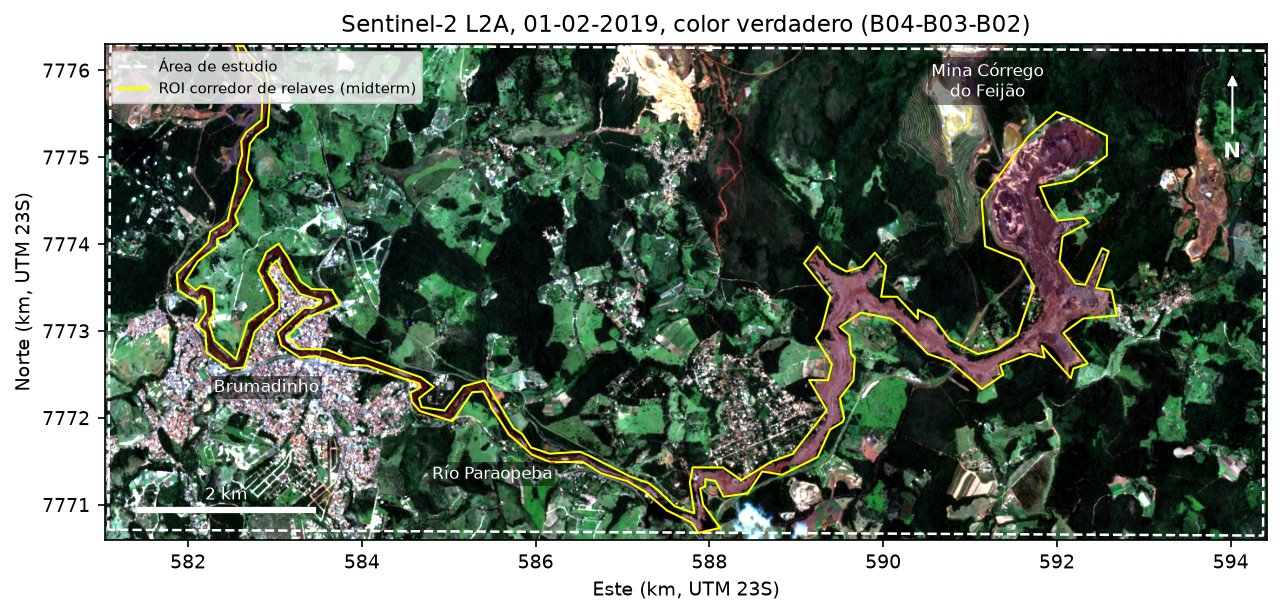
\includegraphics[width=\textwidth]{figures/area_estudio_tc}
 \caption{Área de estudio (línea blanca discontinua) y corredor del relave (amarillo) sobre la escena Sentinel-2 del 1 de febrero de 2019 en color verdadero.}
 \label{fig:area}
\end{figure}

\section{Imagen satelital}

\subsection{Selección y adquisición}
La escena se buscó en el catálogo STAC de Microsoft Planetary Computer \parencite{PlanetaryComputer}, en la colección \texttt{sentinel-2-l2a}. El criterio fue que la escena fuera del 1 de febrero de 2019 y cubriera por completo el área de estudio, y solo una cumplió ambas condiciones. Es la misma adquisición del satélite Sentinel-2A usada en el trabajo anterior; sus metadatos se resumen en la Tabla~\ref{tab:meta}.

Se cambió la fuente de descarga, que antes era Copernicus Browser, porque este proyecto exige al menos diez bandas. El catálogo STAC permite leer las doce bandas directamente desde archivos \emph{Cloud-Optimized GeoTIFF} y descargar solo la ventana del área de estudio.

\begin{table}[htbp]
 \centering
 \small
 \caption{Metadatos de la escena utilizada.}
 \label{tab:meta}
 \begin{tabularx}{\textwidth}{lX}
  \toprule
  Campo & Valor \\
  \midrule
  Identificador del producto & \texttt{S2A\_\allowbreak{}MSIL2A\_\allowbreak{}20190201T131241\_\allowbreak{}N0212\_\allowbreak{}R138\_\allowbreak{}T23KNT\_\allowbreak{}20201007T130407.SAFE} \\
  Plataforma / sensor & Sentinel-2A / MSI \\
  Nivel de procesamiento & L2A (Sen2Cor), reflectancia BOA \\
  \emph{Processing baseline} & 02.12 \\
  Fecha y hora de adquisición (UTC) & 2019-02-01 13:12:41 \\
  Tile MGRS / órbita relativa & 23KNT / R138 (descendente) \\
  Nubosidad de la escena completa & 1{,}14\,\% \\
  Píxeles inválidos (SCL) en el área & 0{,}11\,\% \\
  Ángulos solares medios & cenital 27{,}1$^\circ$, azimut 87{,}8$^\circ$ \\
  SRC del stack & WGS 84 / UTM zona 23S (EPSG:32723) \\
  Tamaño de píxel & 10\,m $\times$ 10\,m \\
  Dimensiones & 1338 columnas $\times$ 570 filas \\
  Tipo de dato / escala & UInt16, reflectancia $\times$ 10\,000 (sin offset) \\
  Fuente & Microsoft Planetary Computer (STAC, \texttt{sentinel-2-l2a}) \\
  \bottomrule
 \end{tabularx}
\end{table}


El producto es de nivel 2A, es decir, reflectancia en la superficie (BOA) corregida atmosféricamente con Sen2Cor \parencite{MainKnorn2017}. En la versión de procesamiento 02.12 no se aplica un desplazamiento radiométrico, por lo que la reflectancia se obtiene como $\rho = DN / 10\,000$.

\subsection{Bandas espectrales}
Se emplearon las doce bandas disponibles en el nivel L2A, listadas en la Tabla~\ref{tab:bandas}. La banda B10, de cirros, solo existe en el nivel L1C. Las bandas de 20 y 60\,m se remuestrearon a 10\,m por interpolación bilineal. Las bandas de 10\,m conservan sus valores originales, porque la malla de salida coincide con la nativa. El resultado es un único GeoTIFF de doce bandas en formato UInt16, que se usa tanto para extraer el conjunto de entrenamiento como para la inferencia de la Fase~3.

\begin{table}[htbp]
 \centering
 \caption{Bandas Sentinel-2 L2A utilizadas \parencite{Drusch2012}.}
 \label{tab:bandas}
 \begin{tabular}{llrrl}
  \toprule
  Banda & Región & $\lambda$ central (nm) & Res. nativa (m) & Remuestreo \\
  \midrule
  B01 & Aerosol costero & 443 & 60 & Bilineal a 10 m \\
  B02 & Azul & 490 & 10 & --- \\
  B03 & Verde & 560 & 10 & --- \\
  B04 & Rojo & 665 & 10 & --- \\
  B05 & Borde rojo 1 & 705 & 20 & Bilineal a 10 m \\
  B06 & Borde rojo 2 & 740 & 20 & Bilineal a 10 m \\
  B07 & Borde rojo 3 & 783 & 20 & Bilineal a 10 m \\
  B08 & NIR & 842 & 10 & --- \\
  B8A & NIR estrecho & 865 & 20 & Bilineal a 10 m \\
  B09 & Vapor de agua & 945 & 60 & Bilineal a 10 m \\
  B11 & SWIR 1 & 1610 & 20 & Bilineal a 10 m \\
  B12 & SWIR 2 & 2190 & 20 & Bilineal a 10 m \\
  \bottomrule
 \end{tabular}
\end{table}


\subsection{Control de calidad}
La capa de clasificación de escena (SCL) se descargó sobre la misma malla, remuestreada por vecino más cercano. Se consideran inválidos los píxeles de las clases 0, 1, 3, 8, 9 y 10: sin datos, saturados, sombra de nube, nubes de probabilidad media y alta, y cirros. Estos píxeles representan el 0{,}11\,\% del área (Figura~\ref{fig:scl}) y se excluyen del conjunto de datos.

La Figura~\ref{fig:fc} presenta dos composiciones en falso color. En ambas el relave se distingue con claridad de la vegetación y del suelo expuesto de la mina.

\begin{figure}[htbp]
 \centering
 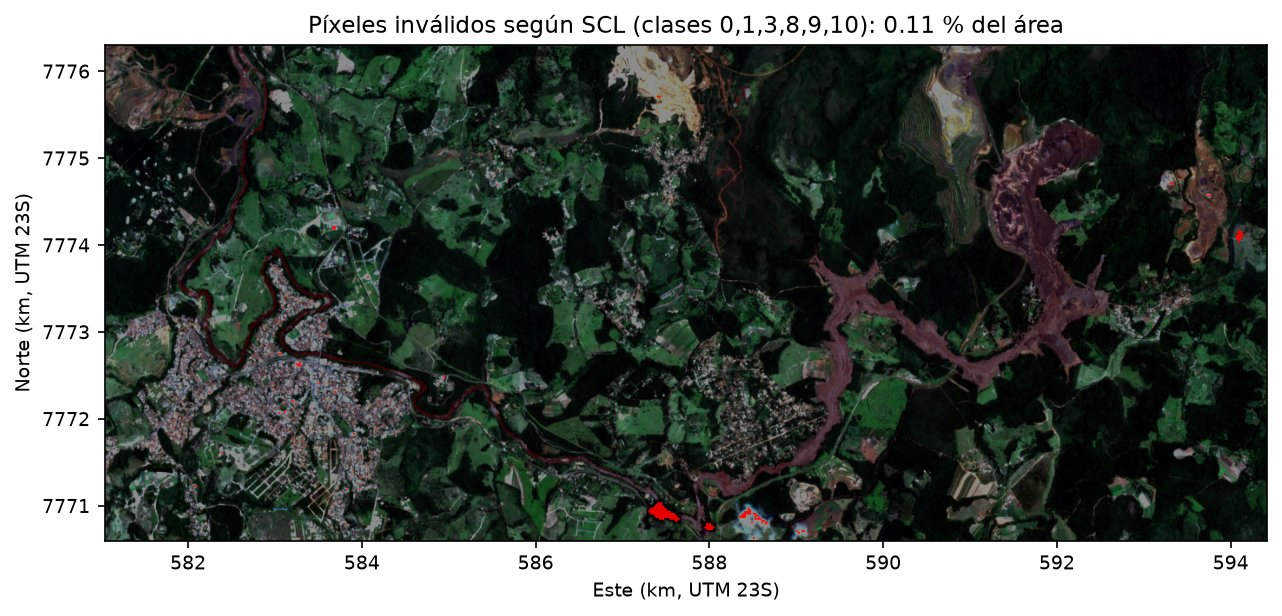
\includegraphics[width=0.9\textwidth]{figures/scl_mask}
 \caption{Píxeles inválidos según la banda SCL, en rojo.}
 \label{fig:scl}
\end{figure}

\begin{figure}[htbp]
 \centering
 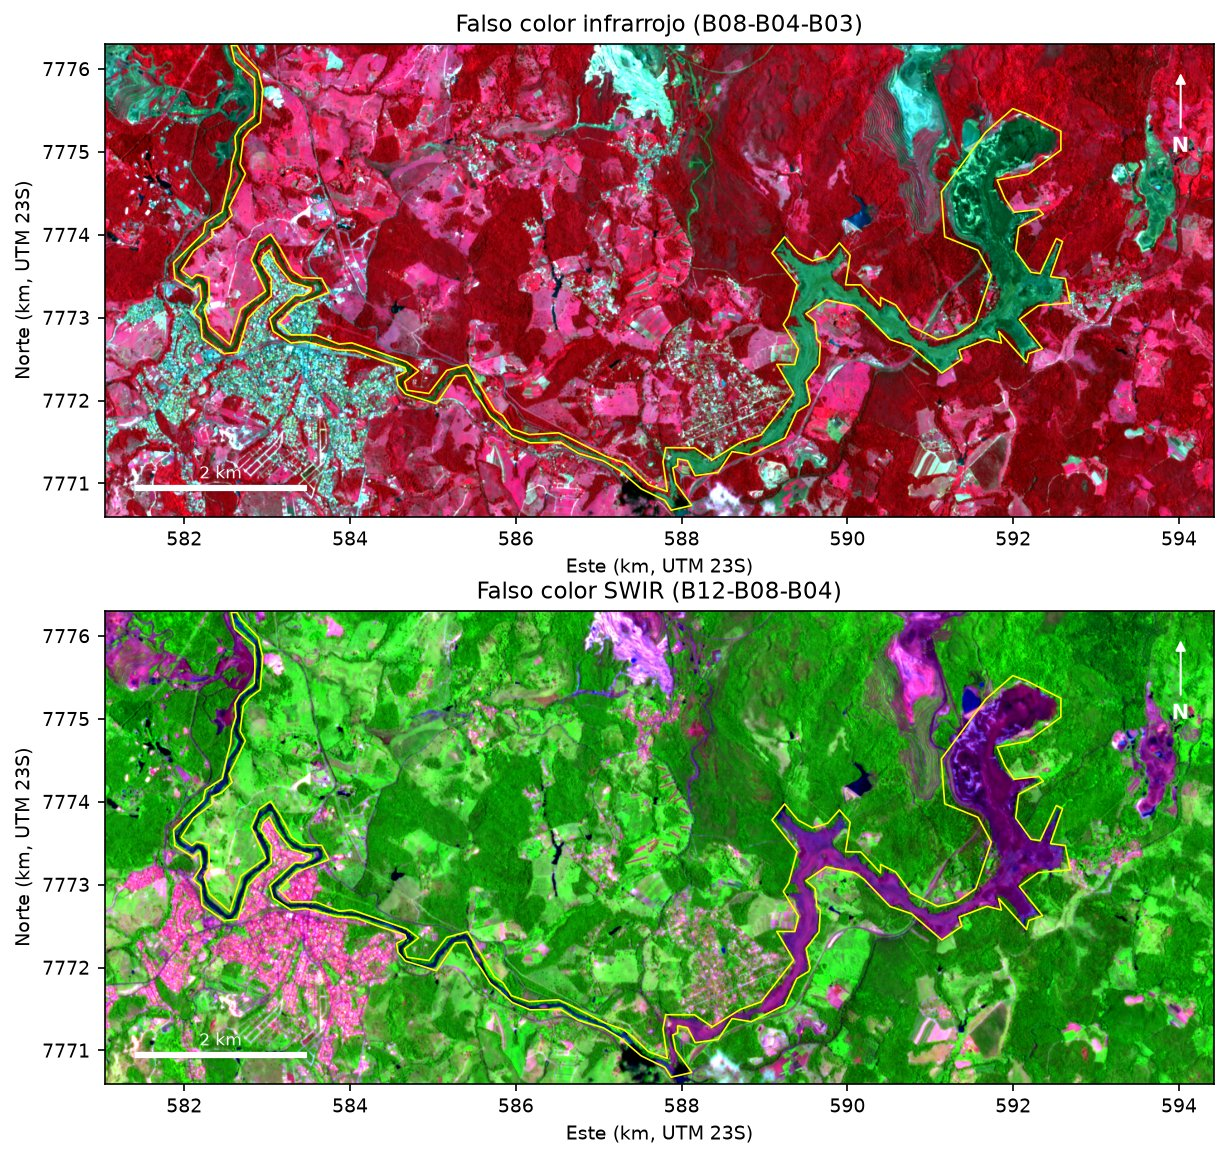
\includegraphics[width=0.9\textwidth]{figures/falso_color}
 \caption{Composiciones en falso color. Arriba, infrarrojo (R=B08, G=B04, B=B03): la vegetación aparece en rojo y el relave en verde oscuro. Abajo, SWIR (R=B12, G=B08, B=B04): el suelo expuesto y las zonas urbanas resaltan en tonos claros.}
 \label{fig:fc}
\end{figure}

\section{Creación del conjunto de datos}

\subsection{Esquema de clases}
Se definieron seis clases de cobertura a partir de la interpretación visual de la escena y de los objetivos del proyecto (Tabla~\ref{tab:clases}). El código numérico de cada clase será el valor del píxel en el ráster temático final.

\begin{table}[htbp]
 \centering
 \caption{Clases de cobertura.}
 \label{tab:clases}
 \begin{tabularx}{\textwidth}{clX}
  \toprule
  Código & Clase & Descripción \\
  \midrule
  1 & Vegetación densa & Bosque atlántico y vegetación arbórea, con NDVI muy alto y SWIR bajo. \\
  2 & Vegetación baja & Pastos, cultivos y vegetación herbácea, con NDVI medio-alto y SWIR alto. \\
  3 & Agua & Cuerpos de agua abiertos: lagunas de la mina y cauces. \\
  4 & Relave minero & Lodo de mineral de hierro depositado por el colapso en el valle del Ribeirão Ferro-Carvão. \\
  5 & Suelo expuesto & Tajos y pilas de la minería, vías sin pavimentar y suelo desnudo. \\
  6 & Urbano & Zonas construidas de Brumadinho y de los núcleos urbanos vecinos. \\
  \bottomrule
 \end{tabularx}
\end{table}

\subsection{Polígonos de entrenamiento}
Como el trabajo anterior solo contaba con el polígono del corredor, se construyó una nueva capa de polígonos de entrenamiento con los campos \texttt{class\_id}, \texttt{class\_name}, \texttt{poly\_id} y \texttt{source}. Se siguió un procedimiento semiautomático en dos pasos.

\paragraph{Propuesta automática.}
Las etiquetas de los polígonos no provienen de visitas de campo, sino de reglas espectrales y espaciales aplicadas sobre la imagen. Primero se calcularon cinco índices espectrales normalizados a partir de las bandas de reflectancia (Tabla~\ref{tab:indices}). Además se usó la diferencia de NDVI ($\Delta$NDVI) calculada en el proyecto de mitad de semestre entre el 17 de enero y el 1 de febrero de 2019.

\begin{table}[htbp]
 \centering
 \small
 \caption{Índices espectrales utilizados para proponer las muestras.}
 \label{tab:indices}
 \begin{tabularx}{\textwidth}{lcX}
  \toprule
  Índice & Fórmula & Qué resalta \\
  \midrule
  NDVI \parencite{Rouse1974} & $\dfrac{B08 - B04}{B08 + B04}$ & Vegetación: aumenta con la densidad y el vigor de las plantas. \\[8pt]
  NDWI \parencite{McFeeters1996} & $\dfrac{B03 - B08}{B03 + B08}$ & Agua abierta. \\[8pt]
  MNDWI \parencite{Xu2006} & $\dfrac{B03 - B11}{B03 + B11}$ & Agua, separándola mejor de las superficies construidas. \\[8pt]
  NDBI \parencite{Zha2003} & $\dfrac{B11 - B08}{B11 + B08}$ & Zonas construidas. \\[8pt]
  BSI \parencite{Rikimaru2002} & $\dfrac{(B11 + B04) - (B08 + B02)}{(B11 + B04) + (B08 + B02)}$ & Suelo desnudo. \\[8pt]
  $\Delta$NDVI & $\mathrm{NDVI}_{t_2} - \mathrm{NDVI}_{t_1}$ & Pérdida de vegetación entre antes y después del colapso. \\
  \bottomrule
 \end{tabularx}
\end{table}

Para cada clase se definió una regla que combina umbrales sobre estos índices, sobre algunas bandas individuales y sobre la ubicación (Tabla~\ref{tab:reglas}). Los umbrales se fijaron a partir de la inspección visual de la escena. Las bandas B11 y B12 se expresan en reflectancia ($DN/10\,000$). \enquote{Fuera del corredor} significa a más de 100\,m del polígono del corredor del relave y fuera de las zonas urbanas.

\begin{table}[htbp]
 \centering
 \small
 \caption{Reglas usadas para proponer las muestras de cada clase.}
 \label{tab:reglas}
 \begin{tabularx}{\textwidth}{lXX}
  \toprule
  Clase & Condición espectral & Restricción espacial \\
  \midrule
  1. Vegetación densa & $\mathrm{NDVI} > 0{,}82$ y $B12 < 0{,}08$ (SWIR bajo, típico del dosel arbóreo) & Fuera del corredor \\
  2. Vegetación baja & $0{,}45 < \mathrm{NDVI} < 0{,}72$ y $B11 > 0{,}20$ (SWIR alto, típico del pasto) & Fuera del corredor \\
  3. Agua & ($\mathrm{SCL} = 6$ o [$\mathrm{MNDWI} > 0{,}2$ y $\mathrm{NDVI} < 0$]) y $\mathrm{NDWI} > 0$ & Ninguna \\
  4. Relave minero & $\Delta\mathrm{NDVI} < -0{,}1$ y $\mathrm{NDVI} < 0{,}25$, sin cumplir la regla de agua & Dentro del corredor del relave \\
  5. Suelo expuesto & $\mathrm{NDVI} < 0{,}20$, $\mathrm{BSI} > 0{,}05$ y $\mathrm{MNDWI} < -0{,}1$ & Fuera del corredor \\
  6. Urbano & $0{,}10 < \mathrm{NDVI} < 0{,}45$ y $\mathrm{NDBI} > -0{,}15$ & Dentro de las zonas urbanas delimitadas visualmente y a más de 100\,m del corredor \\
  \bottomrule
 \end{tabularx}
\end{table}

Las zonas urbanas se delimitaron como dos rectángulos en UTM 23S: el casco de Brumadinho (E 581\,300--584\,600\,m; N 7\,771\,200--7\,773\,300\,m) y el núcleo urbano al sur del corredor (E 587\,300--588\,900\,m; N 7\,771\,400--7\,772\,900\,m). En todas las clases se excluyeron los píxeles marcados como inválidos por la SCL.

A partir de los píxeles que cumplen cada regla se seleccionaron parcelas cuadradas alineadas a la malla, con estos criterios:
\begin{itemize}
 \item \textbf{Tamaño:} $5 \times 5$ píxeles (50\,m de lado) en general, y $3 \times 3$ píxeles (30\,m) para agua y urbano, porque los cuerpos de agua son estrechos y la zona urbana es heterogénea.
 \item \textbf{Pureza:} todos los píxeles de la parcela deben cumplir la regla de su clase.
 \item \textbf{Homogeneidad:} se priorizan las parcelas con menor desviación estándar interna de NDVI, para evitar bordes y coberturas mixtas.
 \item \textbf{Separación mínima:} 400\,m entre parcelas de vegetación, 250\,m en suelo expuesto y urbano, 200\,m en relave y 60\,m en agua. Así las muestras cubren toda el área y se reduce la autocorrelación espacial \parencite{Congalton1991}.
\end{itemize}
Se seleccionaron 12 parcelas por clase.

\paragraph{Revisión visual.}
Las parcelas propuestas se inspeccionaron en conjunto en QGIS sobre las composiciones en color verdadero y en falso color. Las 72 parcelas originales no tuvieron una revisión individual parcela por parcela (campo \texttt{source} = \texttt{borrador}); esa revisión queda pendiente para la Fase~3.

El resultado inicial fueron 72 parcelas, 12 por clase.

\paragraph{Ampliación y revisión.}
Después de la evaluación inicial de la Fase~2 se retiraron \texttt{5\_03} y \texttt{5\_11}. Eran los dos polígonos de prueba de suelo que la SVM clasificaba completos como urbano y como relave, y al revisarlos se consideraron ambiguos entre esas clases. Además se añadieron candidatos propuestos con la misma lógica espectral, exigiendo homogeneidad interna y ausencia de solapes: \texttt{3\_13}--\texttt{3\_18} (agua), \texttt{5\_13}--\texttt{5\_19} (suelo) y \texttt{6\_13}, \texttt{6\_15}, \texttt{6\_16}, \texttt{6\_17} y \texttt{6\_20} (urbano). Los candidatos de agua y urbano se revisaron visualmente (\texttt{source} = \texttt{revisado}); los de suelo no tuvieron revisión individual (\texttt{source} = \texttt{candidato}). El conjunto final tiene 88 parcelas: 12 de vegetación densa, 12 de vegetación baja, 18 de agua, 12 de relave, 17 de suelo expuesto y 17 de urbano (Figuras~\ref{fig:poligonos} y~\ref{fig:zoom}).

Cinco candidatos no respetan la separación mínima descrita arriba: \texttt{3\_13}, \texttt{3\_15} y \texttt{3\_17} quedaron a 10\,m de los polígonos de prueba \texttt{3\_02}, \texttt{3\_06} y \texttt{3\_08}, por la estrechez del cauce; \texttt{5\_16} quedó a 40\,m de \texttt{5\_05}, y \texttt{6\_17} a 60\,m de \texttt{6\_01}. Se comprobó que entrenar sin ellos no cambia la exactitud global de la regresión logística ni de la SVM, así que no inflan el resultado, pero se reporta como limitación de autocorrelación espacial.

\begin{figure}[htbp]
 \centering
 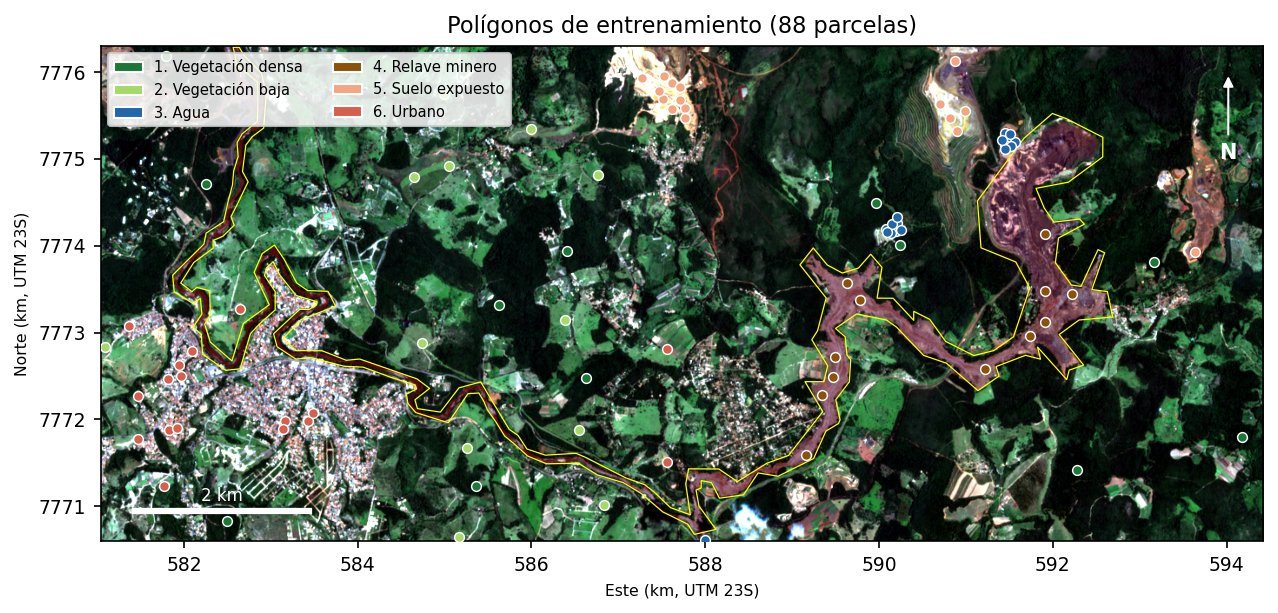
\includegraphics[width=\textwidth]{figures/poligonos_entrenamiento}
 \caption{Distribución de los polígonos de entrenamiento. Los puntos marcan el centro de cada parcela.}
 \label{fig:poligonos}
\end{figure}

\begin{figure}[htbp]
 \centering
 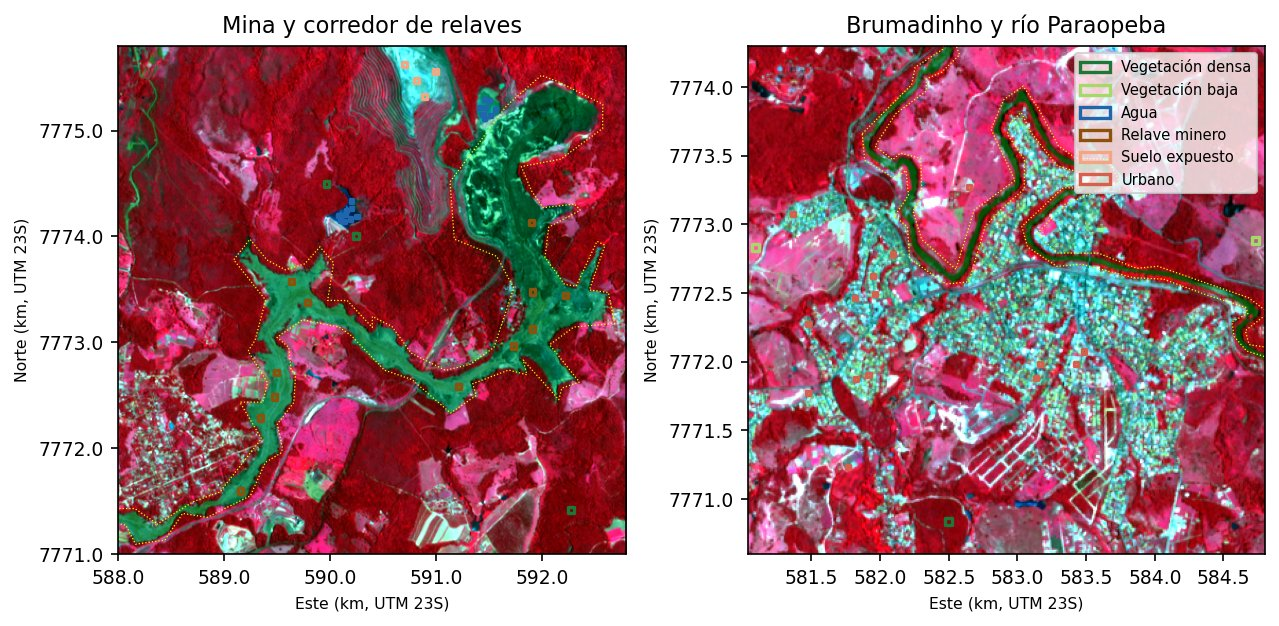
\includegraphics[width=\textwidth]{figures/poligonos_zoom}
 \caption{Detalle de los polígonos sobre la composición en falso color infrarrojo: corredor del relave (izquierda) y casco urbano de Brumadinho (derecha).}
 \label{fig:zoom}
\end{figure}

\subsection{Extracción de píxeles}
Los polígonos se rasterizan sobre la malla de la imagen, y se toma cada píxel cuyo centro cae dentro de un polígono. Se descartan los píxeles inválidos según la SCL y los que no tienen datos. Para cada píxel se calculan las coordenadas de su centro, que se transforman de UTM 23S a WGS84, y se leen los valores de las doce bandas.

Con estos datos se construye el archivo \texttt{training\_dataset.tsv}, separado por tabulaciones, en el que cada fila corresponde a un píxel. Sus columnas se describen en la Tabla~\ref{tab:columnas}, y la Tabla~\ref{tab:muestra} muestra un ejemplo por clase.

\begin{table}[htbp]
 \centering
 \caption{Estructura del archivo \texttt{training\_dataset.tsv} (17 columnas).}
 \label{tab:columnas}
 \begin{tabularx}{\textwidth}{lX}
  \toprule
  Columna & Contenido \\
  \midrule
  \texttt{Latitude}, \texttt{Longitude} & Centro del píxel en grados decimales (WGS84, EPSG:4326). \\
  \texttt{B01}--\texttt{B12} & Reflectancia de superficie $\times$ 10\,000 de las doce bandas (B01--B09, B8A, B11 y B12). \\
  \texttt{class\_id} & Código de la clase (1--6), igual al valor del ráster temático final. \\
  \texttt{class\_name} & Nombre de la clase. \\
  \texttt{poly\_id} & Identificador del polígono de origen. Permite separar entrenamiento y validación por polígono, de modo que píxeles vecinos no queden en ambos conjuntos. \\
  \bottomrule
 \end{tabularx}
\end{table}

\begin{table}[htbp]
 \centering
 \scriptsize
\setlength{\tabcolsep}{2.5pt}
 \caption{Primeras filas del TSV (una por clase).}
 \label{tab:muestra}
 \begin{tabular}{rrrrrrrrrrrrrrl}
  \toprule
  Lat & Lon & B01 & B02 & B03 & B04 & B05 & B06 & B07 & B08 & B8A & B09 & B11 & B12 & Clase \\
  \midrule
  -20{,}12967 & -44{,}17314 & 142 & 154 & 351 & 196 & 669 & 2087 & 2597 & 2632 & 2848 & 2824 & 1470 & 616 & Vegetacion densa \\
  -20{,}13681 & -44{,}17330 & 345 & 477 & 997 & 808 & 1708 & 2890 & 3190 & 3282 & 3509 & 3492 & 2656 & 1406 & Vegetacion baja \\
  -20{,}11796 & -44{,}12489 & 284 & 334 & 761 & 1074 & 1045 & 437 & 436 & 369 & 265 & 320 & 138 & 116 & Agua \\
  -20{,}12761 & -44{,}12054 & 301 & 296 & 416 & 656 & 783 & 865 & 879 & 772 & 806 & 850 & 1299 & 1184 & Relave minero \\
  -20{,}11380 & -44{,}16261 & 616 & 818 & 1450 & 2300 & 2526 & 2668 & 2602 & 2374 & 2316 & 2228 & 2750 & 2137 & Suelo expuesto \\
  -20{,}14857 & -44{,}21696 & 617 & 567 & 960 & 1814 & 1921 & 2314 & 2407 & 2472 & 2472 & 2403 & 3567 & 3211 & Urbano \\
  \bottomrule
 \end{tabular}
\end{table}


\subsection{Resumen del conjunto de datos}
La Tabla~\ref{tab:conteo} resume el número de polígonos y de píxeles por clase. El agua y el urbano siguen teniendo menos píxeles que la vegetación y el relave porque usan parcelas de $3 \times 3$ píxeles: los cuerpos de agua del área son estrechos y la zona urbana es heterogénea a 10\,m de resolución. La ampliación elevó el agua a 18 parcelas y el urbano a 17. Este desbalance se trata en la Fase~2 mediante pesos por clase y el uso de métricas como F1 y Kappa, además de la exactitud global.

\begin{table}[htbp]
 \centering
 \caption{Polígonos y píxeles por clase en \texttt{training\_dataset.tsv}.}
 \label{tab:conteo}
 \begin{tabular}{clrrr}
  \toprule
  Código & Clase & Polígonos & Píxeles & \% \\
  \midrule
  1 & Vegetación densa & 12 & 300 & 18{,}3\,\% \\
  2 & Vegetación baja & 12 & 300 & 18{,}3\,\% \\
  3 & Agua & 18 & 162 & 9{,}9\,\% \\
  4 & Relave minero & 12 & 300 & 18{,}3\,\% \\
  5 & Suelo expuesto & 17 & 425 & 25{,}9\,\% \\
  6 & Urbano & 17 & 153 & 9{,}3\,\% \\
  \midrule
   & \textbf{Total} & 88 & 1640 & 100\,\% \\
  \bottomrule
 \end{tabular}
\end{table}


La Figura~\ref{fig:firmas} presenta la firma espectral por polígono (mediana e IQR entre polígonos) y muestra que las clases son, en general, separables:
\begin{itemize}
 \item las dos clases de vegetación presentan el aumento característico en el borde rojo (B05--B07) y se diferencian por su nivel en el infrarrojo cercano y en el SWIR;
 \item el agua tiene reflectancia baja en el infrarrojo cercano y en el SWIR;
 \item el relave muestra una firma plana, de nivel bajo a medio, distinta de la del suelo expuesto de la mina, que es más brillante en el visible y en el SWIR;
 \item las clases urbano y suelo expuesto son las más parecidas, por lo que es previsible que se confundan; esto justifica comparar modelos no lineales en la Fase~2.
\end{itemize}

\begin{figure}[htbp]
 \centering
 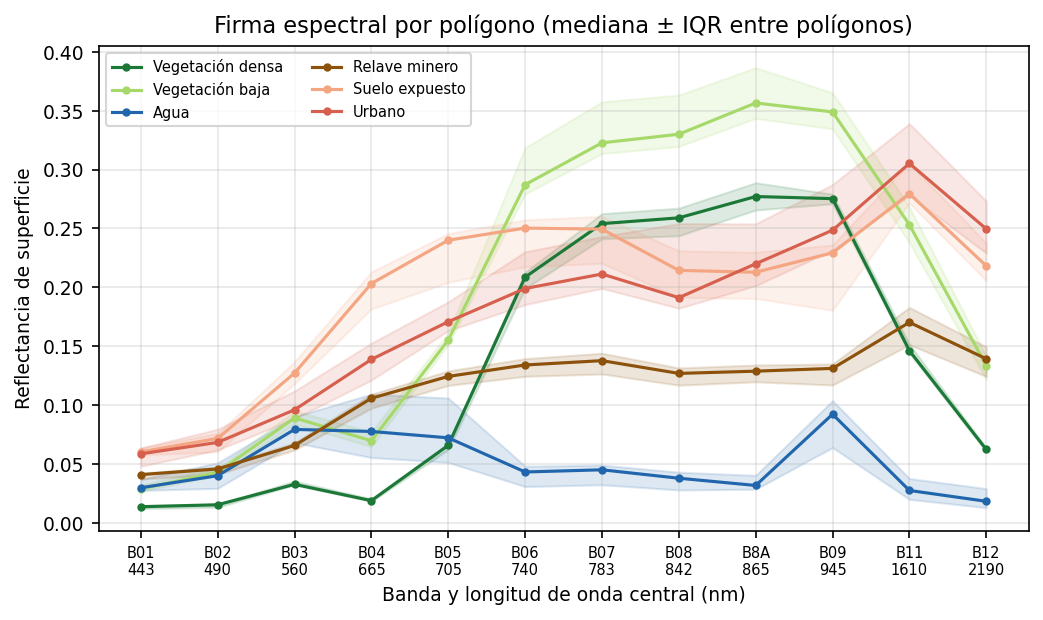
\includegraphics[width=0.85\textwidth]{figures/firmas_espectrales}
 \caption{Firma espectral por polígono: mediana e IQR entre polígonos de cada clase.}
 \label{fig:firmas}
\end{figure}

\part{Fase 2: preprocesamiento y entrenamiento}
\label{part:fase2}

\section{Documentación del archivo TSV}

\subsection{Estructura y contenido}
El archivo \texttt{training\_dataset.tsv} es una tabla de texto separada por tabulaciones con 1640 filas y 17 columnas. Cada fila corresponde a un píxel de 10\,m ubicado dentro de un polígono de entrenamiento, y sus columnas son:
\begin{itemize}
 \item \texttt{Latitude} y \texttt{Longitude}: coordenadas del centro del píxel en WGS84;
 \item \texttt{B01} a \texttt{B12}: los valores de las doce bandas de Sentinel-2 L2A, como reflectancia de superficie multiplicada por 10\,000;
 \item \texttt{class\_id} y \texttt{class\_name}: el código (1--6) y el nombre de la clase;
 \item \texttt{poly\_id}: el identificador del polígono de origen.
\end{itemize}
La Tabla~\ref{tab:conteo} resume el número de polígonos y de píxeles por clase.


\subsection{Control de calidad}
Antes de entrenar se verificó la integridad del archivo y de las geometrías:
\begin{itemize}
 \item no hay valores nulos ni filas duplicadas;
 \item no hay píxeles con coordenadas repetidas;
 \item todos los valores espectrales están entre 79 y 4674 (reflectancia entre 0{,}008 y 0{,}467), un rango físicamente plausible;
 \item no hay píxeles marcados como nube, sombra o sin datos según la banda SCL, porque se descartaron al construir el archivo;
 \item cada \texttt{class\_id} coincide con su \texttt{class\_name} y con la tabla de clases;
 \item no hay solapes entre polígonos y todas las geometrías son válidas.
\end{itemize}

\subsection{Estadística descriptiva}
La Tabla~\ref{tab:estadistica} presenta la media y la desviación estándar por píxel de cada banda por clase. La Figura~\ref{fig:firmas} resume la firma espectral por polígono con la mediana y el rango intercuartílico (IQR) entre polígonos. La vegetación densa y la baja se distinguen por su nivel en el infrarrojo cercano (B08, B8A) y en el SWIR (B11, B12). El agua es la única clase con reflectancia muy baja en el infrarrojo. Las clases urbano y suelo expuesto tienen las firmas más parecidas, lo que anticipa confusiones entre ellas.

\begin{table}[htbp]
 \centering
 \footnotesize
\setlength{\tabcolsep}{4pt}
 \caption{Media $\pm$ desviación estándar de cada banda por clase en \texttt{training\_dataset.tsv} (reflectancia $\times$ 10\,000).}
 \label{tab:estadistica}
 \begin{tabular}{lrrrrrr}
  \toprule
  Banda & Veg. densa & Veg. baja & Agua & Relave & Suelo exp. & Urbano \\
  \midrule
  B01 & 136 $\pm$ 15 & 295 $\pm$ 42 & 314 $\pm$ 65 & 390 $\pm$ 47 & 627 $\pm$ 142 & 566 $\pm$ 124 \\
  B02 & 147 $\pm$ 20 & 429 $\pm$ 42 & 402 $\pm$ 139 & 433 $\pm$ 76 & 726 $\pm$ 197 & 712 $\pm$ 197 \\
  B03 & 335 $\pm$ 38 & 887 $\pm$ 64 & 789 $\pm$ 152 & 621 $\pm$ 98 & 1255 $\pm$ 266 & 1013 $\pm$ 237 \\
  B04 & 190 $\pm$ 17 & 704 $\pm$ 69 & 811 $\pm$ 322 & 1000 $\pm$ 165 & 1923 $\pm$ 437 & 1454 $\pm$ 335 \\
  B05 & 655 $\pm$ 59 & 1552 $\pm$ 98 & 785 $\pm$ 315 & 1178 $\pm$ 191 & 2214 $\pm$ 466 & 1795 $\pm$ 313 \\
  B06 & 2112 $\pm$ 245 & 2954 $\pm$ 258 & 414 $\pm$ 155 & 1268 $\pm$ 205 & 2336 $\pm$ 468 & 2141 $\pm$ 419 \\
  B07 & 2592 $\pm$ 319 & 3317 $\pm$ 299 & 435 $\pm$ 157 & 1293 $\pm$ 212 & 2331 $\pm$ 454 & 2287 $\pm$ 466 \\
  B08 & 2636 $\pm$ 347 & 3374 $\pm$ 295 & 367 $\pm$ 148 & 1186 $\pm$ 209 & 2081 $\pm$ 451 & 2166 $\pm$ 566 \\
  B8A & 2836 $\pm$ 331 & 3619 $\pm$ 294 & 342 $\pm$ 124 & 1204 $\pm$ 203 & 2079 $\pm$ 448 & 2383 $\pm$ 485 \\
  B09 & 2809 $\pm$ 263 & 3509 $\pm$ 268 & 876 $\pm$ 285 & 1228 $\pm$ 189 & 2137 $\pm$ 437 & 2593 $\pm$ 383 \\
  B11 & 1483 $\pm$ 81 & 2529 $\pm$ 184 & 294 $\pm$ 124 & 1656 $\pm$ 233 & 2803 $\pm$ 635 & 3099 $\pm$ 462 \\
  B12 & 630 $\pm$ 40 & 1325 $\pm$ 131 & 211 $\pm$ 97 & 1399 $\pm$ 178 & 2217 $\pm$ 469 & 2500 $\pm$ 553 \\
  \bottomrule
 \end{tabular}
\end{table}


\subsection{Preprocesamiento}
Sobre el TSV se aplicaron dos transformaciones antes de entrenar:
\begin{enumerate}
 \item \textbf{Conversión a reflectancia:} los valores de las bandas se dividieron entre 10\,000.
 \item \textbf{Estandarización:} cada variable se transformó a media 0 y desviación estándar 1 con \texttt{StandardScaler}. El estandarizador se ajustó únicamente con los datos de entrenamiento y se aplicó después a los de prueba, para no filtrar información del conjunto de prueba.
\end{enumerate}
Para la pista B se construyó un dataset auxiliar con una fila por polígono: mediana de cada banda, IQR, número de píxeles e índices NDVI, NDWI, MNDWI, NDBI y BSI. Esos 17 valores (12 bandas y 5 índices) son las variables de la pista B.

\section{Metodología}

\subsection{División en entrenamiento y prueba}
Los píxeles de un mismo polígono son vecinos y casi idénticos entre sí. Si se repartieran al azar entre entrenamiento y prueba, el modelo se evaluaría con píxeles prácticamente iguales a los que ya vio y las métricas quedarían infladas \parencite{Roberts2017}. Por eso la división se hizo \textbf{por polígono}: en cada clase se eligieron al azar 4 de los polígonos originales para prueba y el resto para entrenamiento, con una semilla fija (42). La prueba son 24 polígonos originales; los polígonos añadidos en la ampliación se usan únicamente para entrenamiento (Tabla~\ref{tab:division} y Figura~\ref{fig:division}). Ningún polígono aparece en ambos conjuntos.

\begin{table}[htbp]
 \centering
 \caption{División del conjunto de datos por polígono.}
 \label{tab:division}
 \begin{tabular}{lrrrr}
  \toprule
  Clase & Polígonos entren. & Píxeles entren. & Polígonos prueba & Píxeles prueba \\
  \midrule
  Vegetación densa & 8 & 200 & 4 & 100 \\
  Vegetación baja & 8 & 200 & 4 & 100 \\
  Agua & 14 & 126 & 4 & 36 \\
  Relave minero & 8 & 200 & 4 & 100 \\
  Suelo expuesto & 13 & 325 & 4 & 100 \\
  Urbano & 13 & 117 & 4 & 36 \\
  \midrule
  Total & 64 & 1168 & 24 & 472 \\
  \bottomrule
 \end{tabular}
\end{table}


\begin{figure}[htbp]
 \centering
 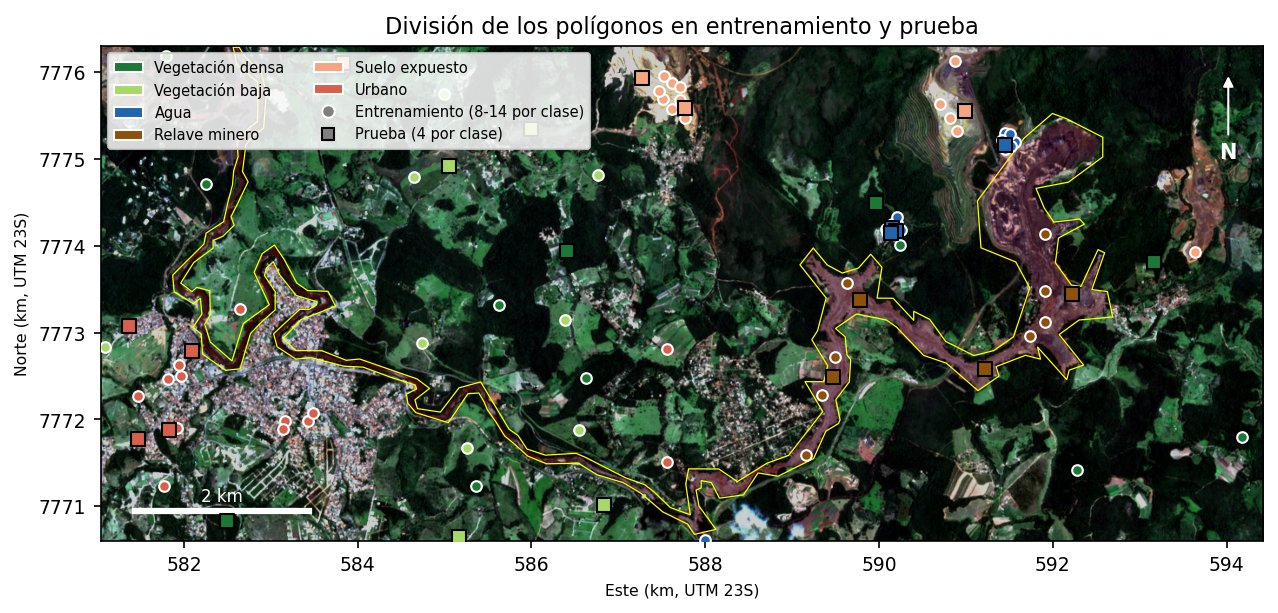
\includegraphics[width=\textwidth]{figures/division_poligonos}
 \caption{Polígonos de entrenamiento (círculos) y de prueba (cuadrados) sobre la imagen en color verdadero.}
 \label{fig:division}
\end{figure}

Este diseño mantiene el mismo conjunto de prueba para vegetación, agua, relave y urbano, pero no para suelo: se retiraron \texttt{5\_03} y \texttt{5\_11}, y la prueba de suelo pasó de \texttt{5\_03}, \texttt{5\_05}, \texttt{5\_10} y \texttt{5\_11} a \texttt{5\_04}, \texttt{5\_05}, \texttt{5\_06} y \texttt{5\_09}. Los dos polígonos retirados eran justamente los que la SVM fallaba, y se retiraron después de ver ese resultado. Una decisión así favorece a los modelos en la prueba actual, por lo que el resultado de referencia de esta fase es el de la \textbf{prueba original} (Sección~\ref{sec:referencia}). La Tabla~\ref{tab:comparacion_pareada} compara ambos entrenamientos sobre el mismo conjunto y separa el efecto de los datos del efecto del test.

Cinco polígonos añadidos quedaron por debajo de la separación mínima de la Fase~1 respecto a polígonos de prueba: \texttt{3\_13}, \texttt{3\_15} y \texttt{3\_17} a 10\,m de \texttt{3\_02}, \texttt{3\_06} y \texttt{3\_08}; \texttt{5\_16} a 40\,m de \texttt{5\_05}, y \texttt{6\_17} a 60\,m de \texttt{6\_01}. Se comprobó que entrenar sin esos cinco polígonos da la misma exactitud global en la regresión logística y en la SVM (94{,}7\,\%), así que su cercanía no infla el resultado.

\subsection{Validación cruzada y estabilidad}
Como complemento a la división única, se usó \texttt{LeaveOneGroupOut}: en cada pliegue se deja fuera un polígono completo y se entrena con los demás. Se reportan la OA y el Kappa out-of-fold, la media y el error estándar de la OA por pliegue, y un intervalo de confianza bootstrap al 95\,\% calculado remuestreando polígonos de prueba estratificados por clase.

\subsection{Modelos}
Se entrenaron los cinco modelos que pide el enunciado, más un Random Forest como complemento del árbol de decisión. La Tabla~\ref{tab:modelos} resume su configuración inicial. En los modelos que lo permiten se usaron pesos por clase (\texttt{class\_weight=balanced}) para compensar el menor número de píxeles de agua y urbano. Para el quinto modelo se eligió KNN, por ser un método no paramétrico que trabaja directamente en el espacio espectral.

\begin{table}[htbp]
 \centering
 \small
 \caption{Modelos y configuración inicial (scikit-learn). En todos, las bandas se estandarizan con \texttt{StandardScaler} ajustado solo con el entrenamiento.}
 \label{tab:modelos}
 \begin{tabularx}{\textwidth}{llX}
  \toprule
   & Modelo & Configuración inicial \\
  \midrule
  LR & Regresión logística & \texttt{max\_iter=1000}, \texttt{class\_weight=balanced} \\
  DT & Árbol de decisión & Sin límite de profundidad, criterio Gini, \texttt{class\_weight=balanced} \\
  RF & Random Forest & 300 árboles, \texttt{class\_weight=balanced} \\
  SVM & Máquina de soporte vectorial & Kernel RBF, $C=1$, $\gamma$ = \texttt{scale}, \texttt{class\_weight=balanced} \\
  ANN & Red neuronal (MLP) & Dos capas ocultas (64 y 32 neuronas), ReLU, Adam, \texttt{max\_iter=2000} \\
  KNN & K vecinos más cercanos & $k=5$, distancia euclidiana, voto uniforme \\
  \bottomrule
 \end{tabularx}
\end{table}


\subsection{Métricas}
Para cada modelo se calcularon dos niveles de evaluación:
\begin{itemize}
 \item \textbf{por píxel:} matriz de confusión, exactitud global (OA), Kappa, precisión, recall y F1;
 \item \textbf{por polígono:} voto mayoritario de las predicciones de sus píxeles, pureza (fracción de píxeles que votan por la clase mayoritaria) y acierto del polígono.
\end{itemize}
La exactitud global y el Kappa se definen como
\begin{equation}
 \mathrm{OA} = \frac{\sum_{i} n_{ii}}{N}, \qquad
 \kappa = \frac{p_o - p_e}{1 - p_e}, \qquad
 p_e = \sum_{i} \frac{n_{i+}\, n_{+i}}{N^2},
\end{equation}
donde $p_o$ es la OA, y $n_{i+}$ y $n_{+i}$ son los totales de la fila y de la columna $i$ \parencite{Cohen1960}. La precisión, el recall y el F1 se calculan por clase; el F1 macro es su promedio simple.

\section{Resultados}

\subsection{Comparación de los modelos por píxel}
Esta sección presenta primero las métricas mínimas de la fase, la exactitud global y las matrices de confusión por píxel sobre la prueba actual, y después el resultado de referencia sobre la prueba original (Sección~\ref{sec:referencia}). La Tabla~\ref{tab:metricas} y la Figura~\ref{fig:metricas} resumen las métricas de los seis modelos. En la prueba actual, la regresión logística y la SVM empatan en la mejor exactitud global (94{,}7\,\%), el mejor Kappa (0{,}935) y el mejor F1 macro (0{,}933). En la validación cruzada, la SVM obtiene la OA out-of-fold más alta (94{,}5\,\%), seguida de la regresión logística (94{,}0\,\%). El árbol de decisión individual es el modelo más débil (86{,}7\,\%), y el Random Forest lo mejora en unos cuatro puntos. La red neuronal queda en 89{,}8\,\%: su resultado es sensible a la composición de la prueba y no supera a los modelos más simples.

\begin{table}[htbp]
 \centering
 \small
\setlength{\tabcolsep}{4pt}
 \caption{Métricas sobre el conjunto de prueba (24 polígonos, 472 píxeles) y OA LOO out-of-fold $\pm$ error estándar de la OA por pliegue. En negrita, el mejor valor.}
 \label{tab:metricas}
 \begin{tabular}{llcccccc}
  \toprule
   & Modelo & OA & Kappa & Precisión & Recall & F1 & OA LOO \\
  \midrule
  LR & Regresión logística & \textbf{0{,}947} & \textbf{0{,}935} & \textbf{0{,}932} & \textbf{0{,}958} & \textbf{0{,}933} & 0{,}940 $\pm$ 0{,}022 \\
  DT & Árbol de decisión & 0{,}867 & 0{,}837 & 0{,}867 & 0{,}889 & 0{,}863 & 0{,}844 $\pm$ 0{,}032 \\
  RF & Random Forest & 0{,}909 & 0{,}888 & 0{,}899 & 0{,}928 & 0{,}903 & 0{,}916 $\pm$ 0{,}025 \\
  SVM & Máquina de soporte vectorial & \textbf{0{,}947} & \textbf{0{,}935} & \textbf{0{,}932} & \textbf{0{,}958} & \textbf{0{,}933} & 0{,}945 $\pm$ 0{,}020 \\
  ANN & Red neuronal (MLP) & 0{,}898 & 0{,}875 & 0{,}893 & 0{,}920 & 0{,}895 & 0{,}930 $\pm$ 0{,}023 \\
  KNN & K vecinos más cercanos & 0{,}892 & 0{,}868 & 0{,}889 & 0{,}915 & 0{,}890 & 0{,}929 $\pm$ 0{,}023 \\
  \bottomrule
 \end{tabular}
\end{table}


\begin{figure}[htbp]
 \centering
 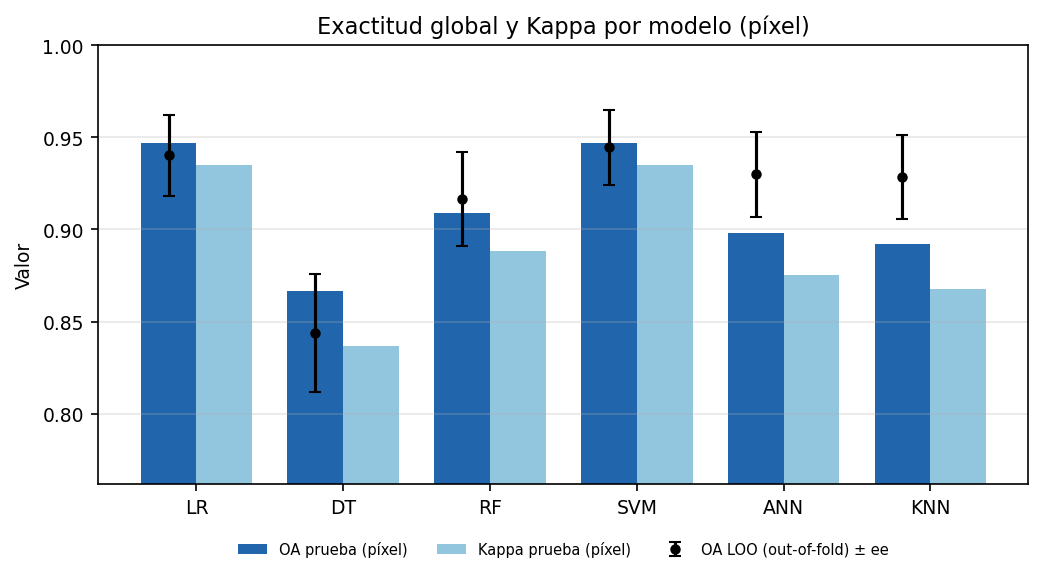
\includegraphics[width=0.85\textwidth]{figures/metricas_modelos}
 \caption{Exactitud global y Kappa sobre el conjunto de prueba, y OA out-of-fold ($\pm$ error estándar) de la validación cruzada.}
 \label{fig:metricas}
\end{figure}

\subsection{Matrices de confusión}
La Figura~\ref{fig:matrices} presenta las matrices de confusión de los seis modelos. La vegetación densa, la vegetación baja, el agua y el relave se clasifican sin errores en la regresión logística y en la SVM. El error restante está en suelo expuesto: uno de los cuatro polígonos de prueba, \texttt{5\_06}, se clasifica completo como urbano (25 píxeles). Por eso el recall de suelo es 0{,}75, la precisión del urbano es 0{,}59 y su F1 es 0{,}742.

\begin{figure}[htbp]
 \centering
 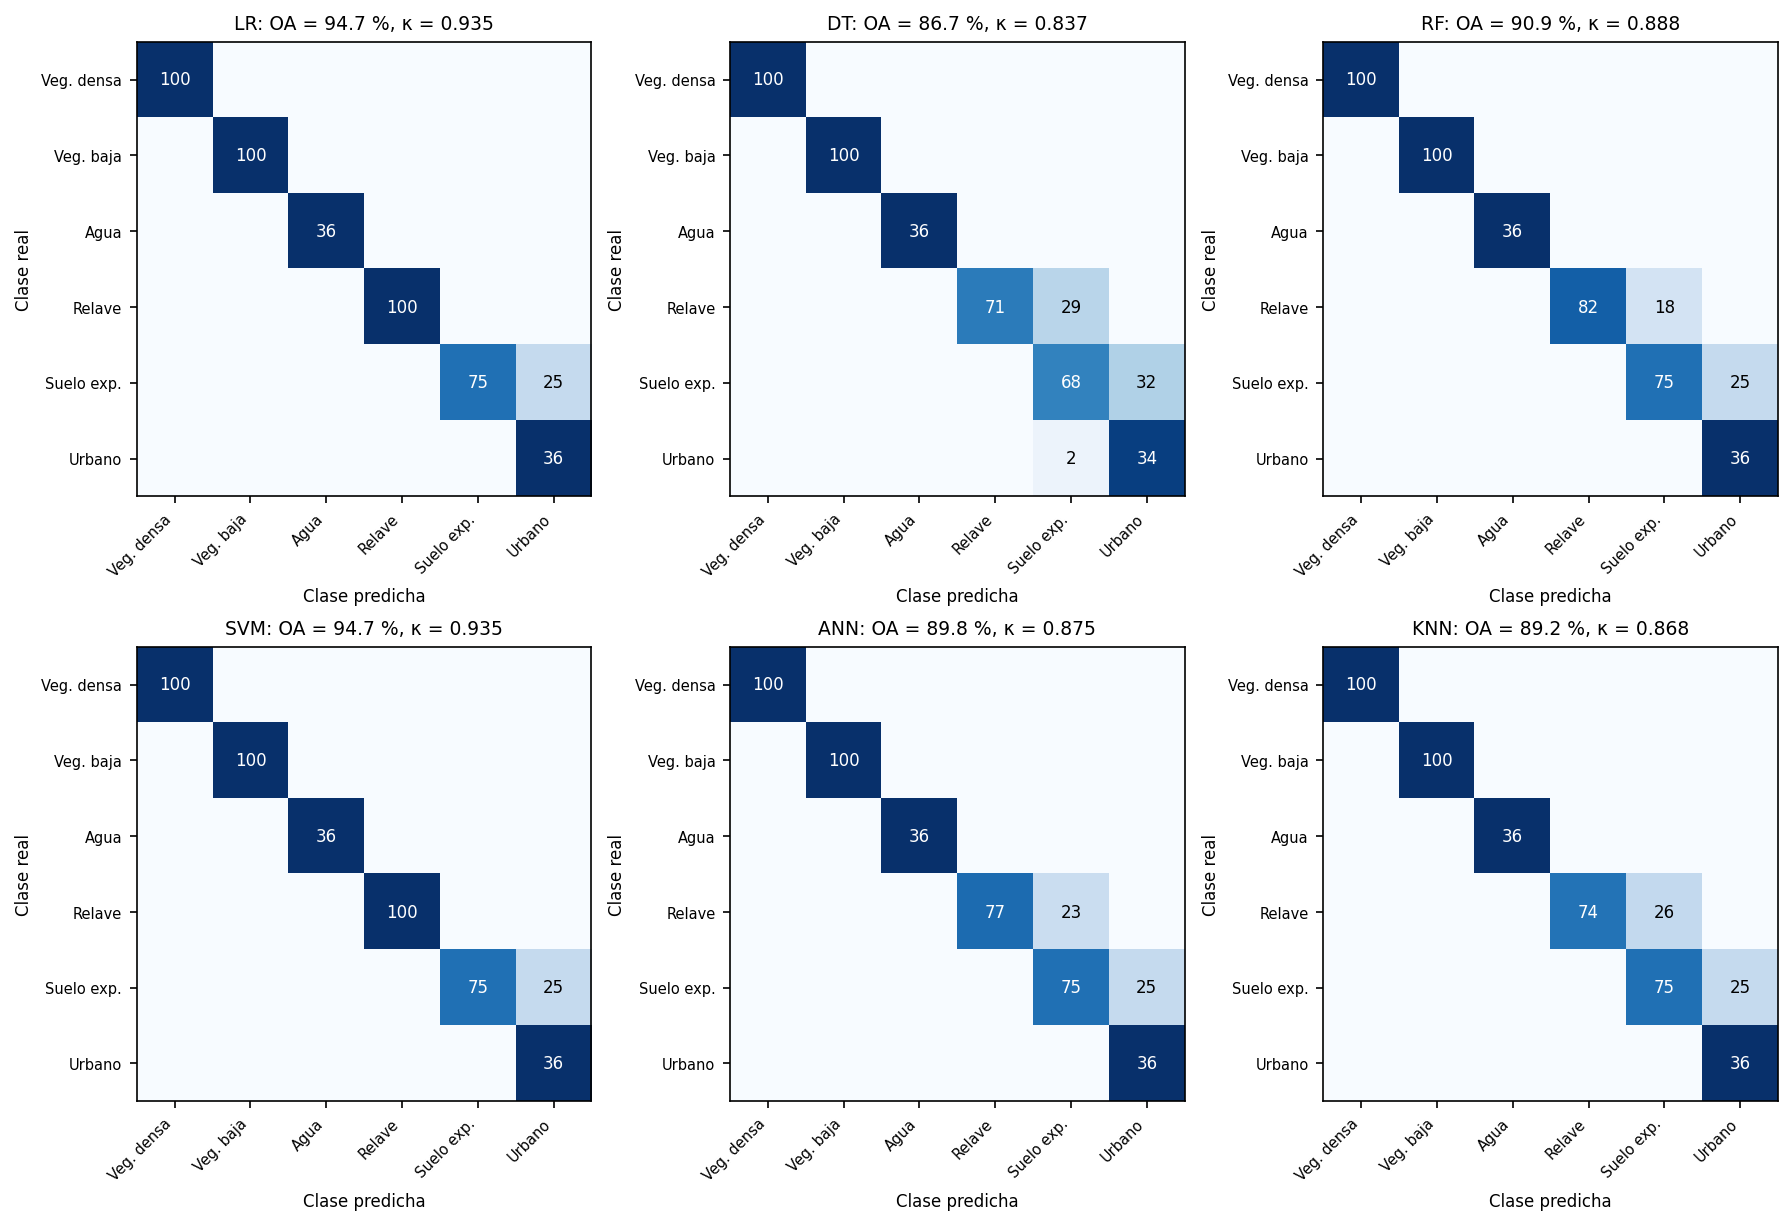
\includegraphics[width=\textwidth]{figures/matrices_confusion}
 \caption{Matrices de confusión por píxel sobre el conjunto de prueba. Los números son píxeles; el color indica la proporción respecto al total de la clase real.}
 \label{fig:matrices}
\end{figure}

La Tabla~\ref{tab:matriz_mejor} muestra la matriz de la regresión logística, que empata con la SVM en todas las métricas, y la Tabla~\ref{tab:por_clase} sus métricas por clase. La red neuronal tiene un error adicional: asigna 23 píxeles de relave a suelo, por lo que su recall de relave baja a 0{,}77 (Tabla~\ref{tab:por_clase}).

\begin{table}[htbp]
 \centering
 \small
\setlength{\tabcolsep}{3.5pt}
 \caption{Matriz de confusión del mejor modelo por píxel (Regresión logística). Filas: clase real; columnas: clase predicha; EP: exactitud del productor; EU: exactitud del usuario.}
 \label{tab:matriz_mejor}
 \begin{tabular}{lrrrrrrrr}
  \toprule
  Real / Predicha & Veg. densa & Veg. baja & Agua & Relave & Suelo exp. & Urbano & Total & EP (\%) \\
  \midrule
  Veg. densa & 100 & 0 & 0 & 0 & 0 & 0 & 100 & 100{,}0 \\
  Veg. baja & 0 & 100 & 0 & 0 & 0 & 0 & 100 & 100{,}0 \\
  Agua & 0 & 0 & 36 & 0 & 0 & 0 & 36 & 100{,}0 \\
  Relave & 0 & 0 & 0 & 100 & 0 & 0 & 100 & 100{,}0 \\
  Suelo exp. & 0 & 0 & 0 & 0 & 75 & 25 & 100 & 75{,}0 \\
  Urbano & 0 & 0 & 0 & 0 & 0 & 36 & 36 & 100{,}0 \\
  \midrule
  Total & 100 & 100 & 36 & 100 & 75 & 61 & 472 & \\
  EU (\%) & 100{,}0 & 100{,}0 & 100{,}0 & 100{,}0 & 100{,}0 & 59{,}0 & & \\
  \bottomrule
 \end{tabular}
\end{table}


\begin{table}[htbp]
 \centering
 \caption{Precisión, recall y F1 por clase del mejor modelo por píxel (Regresión logística).}
 \label{tab:por_clase}
 \begin{tabular}{lcccr}
  \toprule
  Clase & Precisión & Recall & F1 & Píxeles de prueba \\
  \midrule
  Vegetación densa & 1{,}000 & 1{,}000 & 1{,}000 & 100 \\
  Vegetación baja & 1{,}000 & 1{,}000 & 1{,}000 & 100 \\
  Agua & 1{,}000 & 1{,}000 & 1{,}000 & 36 \\
  Relave minero & 1{,}000 & 1{,}000 & 1{,}000 & 100 \\
  Suelo expuesto & 1{,}000 & 0{,}750 & 0{,}857 & 100 \\
  Urbano & 0{,}590 & 1{,}000 & 0{,}742 & 36 \\
  \bottomrule
 \end{tabular}
\end{table}


\subsection{Resultado de referencia: prueba original}
\label{sec:referencia}
La Tabla~\ref{tab:comparacion_pareada} compara el entrenamiento con 72 polígonos (base) y con 88 (nuevo) sobre el mismo conjunto de prueba. En la \textbf{prueba original}, definida antes de la ampliación y que incluye \texttt{5\_03} y \texttt{5\_11}, la SVM se mantiene en 0{,}894 y la regresión logística sube de 0{,}883 a 0{,}894. Este es el resultado de referencia de la fase: la ampliación apenas cambia el desempeño. En la prueba actual, la SVM sube 4{,}9 puntos y la regresión logística 0{,}4, y en los 22 polígonos comunes a ambas pruebas los dos modelos son casi perfectos. Por tanto, la diferencia entre 89{,}4\,\% y 94{,}7\,\% se debe sobre todo a la composición de la prueba de suelo, no a los datos nuevos.

\begin{table}[htbp]
 \centering
 \small
 \setlength{\tabcolsep}{4pt}
 \caption{Comparación pareada del efecto de la ampliación (OA). \emph{Original 24}: test de la versión de 72 polígonos. \emph{Nuevo 24}: test de la versión de 88. \emph{Común 22}: test original sin \texttt{5\_03} ni \texttt{5\_11}. La base del test nuevo se entrena solo con polígonos originales que no están en ese test, para evitar fuga.}
 \label{tab:comparacion_pareada}
 \begin{tabular}{lcccc}
  \toprule
  Test & Modelo & Base & Nuevo & $\Delta$ \\
  \midrule
  Original 24 & LR & 0{,}883 & 0{,}894 & $+0{,}011$ \\
  Original 24 & SVM & 0{,}894 & 0{,}894 & $0{,}000$ \\
  Nuevo 24 & LR & 0{,}943 & 0{,}947 & $+0{,}004$ \\
  Nuevo 24 & SVM & 0{,}898 & 0{,}947 & $+0{,}049$ \\
  Común 22 & LR & 0{,}988 & 1{,}000 & $+0{,}012$ \\
  Común 22 & SVM & 1{,}000 & 1{,}000 & $0{,}000$ \\
  \bottomrule
 \end{tabular}
\end{table}


\subsection{Evaluación por polígono}
La Figura~\ref{fig:matrices_pol} presenta las matrices de confusión por polígono de la pista B (medianas por polígono) y la Tabla~\ref{tab:metricas_poligono} compara las dos pistas. En la pista A, la regresión logística y la SVM aciertan 23 de los 24 polígonos de prueba (OA 0{,}958, Kappa 0{,}950); el único error es \texttt{5\_06}. En la pista B, la regresión logística y el Random Forest también alcanzan 0{,}958/0{,}950. Las diferencias entre modelos son de uno o dos polígonos, por lo que no son concluyentes.

\begin{figure}[htbp]
 \centering
 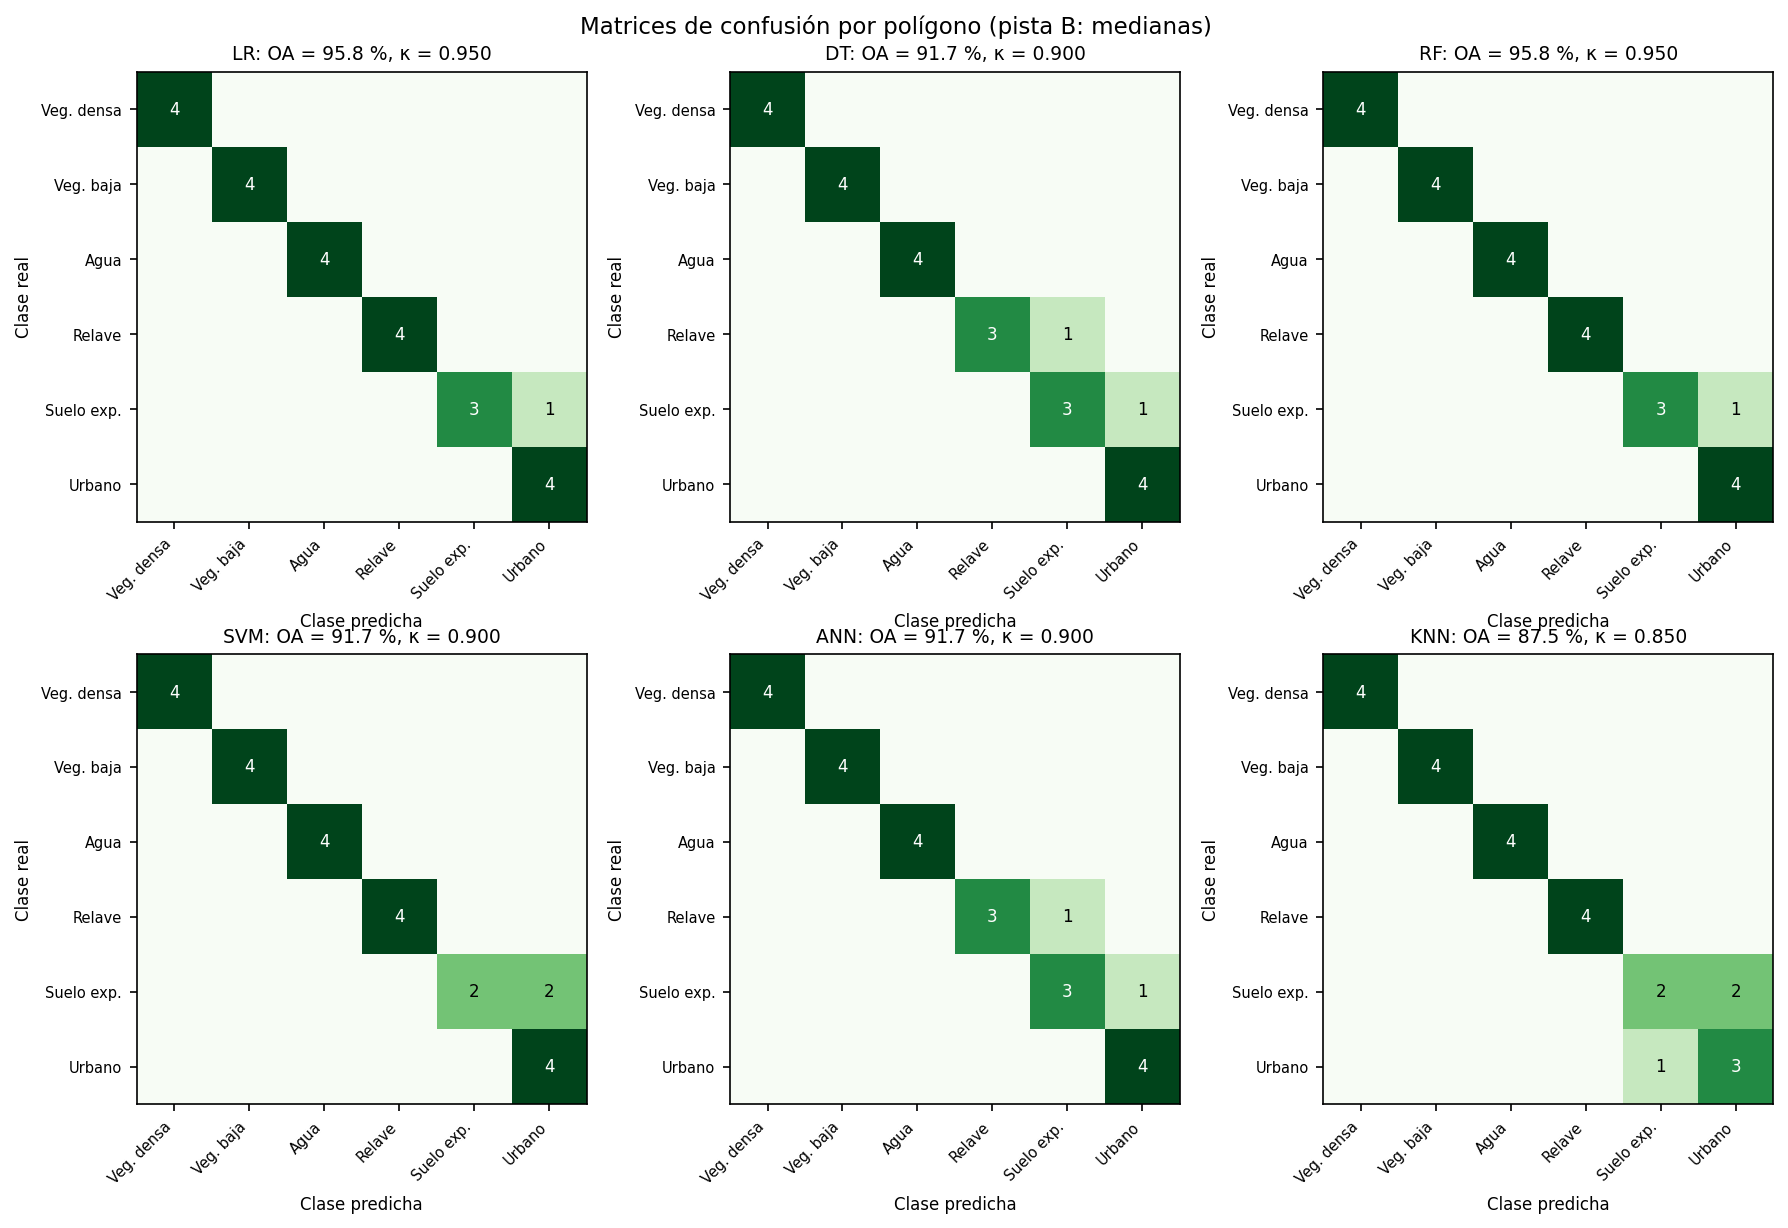
\includegraphics[width=\textwidth]{figures/matrices_confusion_poligono}
 \caption{Matrices de confusión por polígono de la pista B (medianas por polígono). Los números son polígonos.}
 \label{fig:matrices_pol}
\end{figure}

\begin{table}[htbp]
 \centering
 \small
\setlength{\tabcolsep}{3.5pt}
 \caption{Métricas por polígono (24 de prueba). Pista A: votación mayoritaria de las predicciones por píxel; pista B: mediana por polígono e índices. Las diferencias de uno o dos polígonos no son concluyentes.}
 \label{tab:metricas_poligono}
 \begin{tabular}{lccccccc}
  \toprule
  Modelo & A OA & A Kappa & A F1 & A pureza & B OA & B Kappa & B F1 \\
  \midrule
  LR & 0{,}958 & 0{,}950 & 0{,}958 & 1{,}000 & 0{,}958 & 0{,}950 & 0{,}958 \\
  DT & 0{,}917 & 0{,}900 & 0{,}916 & 0{,}972 & 0{,}917 & 0{,}900 & 0{,}916 \\
  RF & 0{,}917 & 0{,}900 & 0{,}916 & 0{,}988 & 0{,}958 & 0{,}950 & 0{,}958 \\
  SVM & 0{,}958 & 0{,}950 & 0{,}958 & 1{,}000 & 0{,}917 & 0{,}900 & 0{,}911 \\
  ANN & 0{,}917 & 0{,}900 & 0{,}916 & 0{,}990 & 0{,}917 & 0{,}900 & 0{,}916 \\
  KNN & 0{,}917 & 0{,}900 & 0{,}916 & 0{,}998 & 0{,}875 & 0{,}850 & 0{,}873 \\
  \bottomrule
 \end{tabular}
\end{table}


\begin{figure}[htbp]
 \centering
 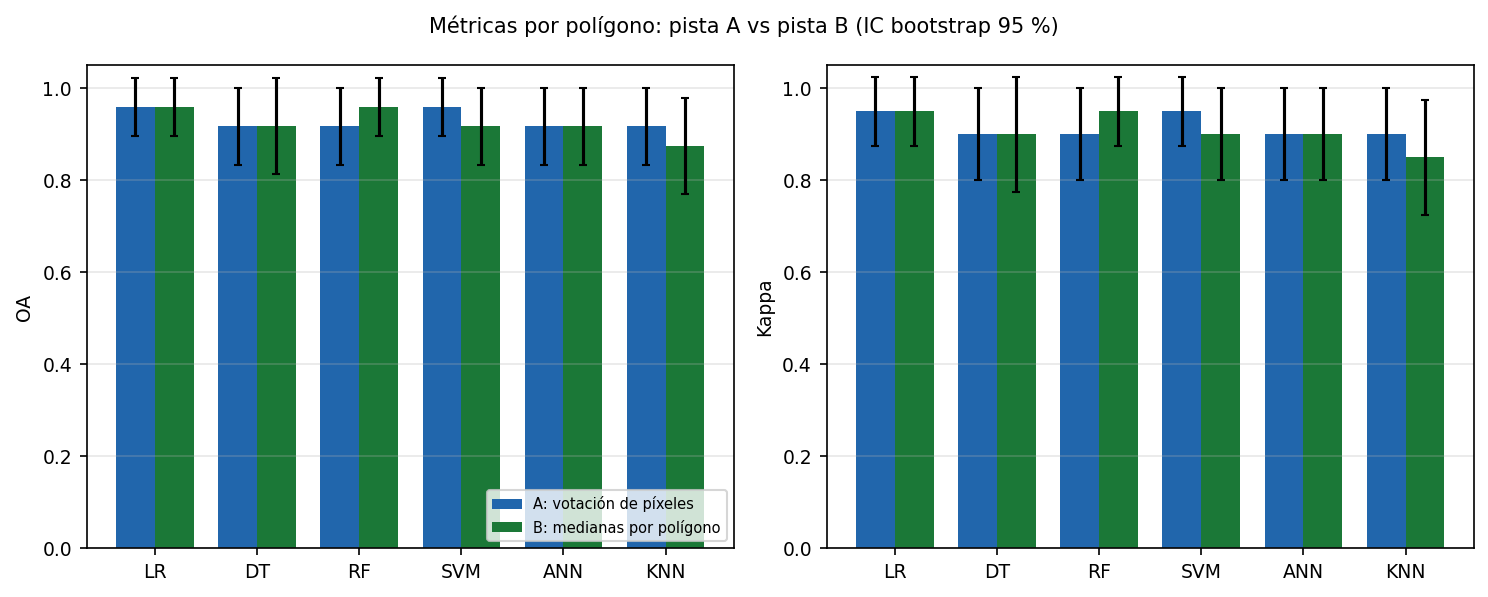
\includegraphics[width=0.95\textwidth]{figures/metricas_poligono}
 \caption{OA y Kappa por polígono de las pistas A y B, con IC bootstrap al 95\,\%.}
 \label{fig:metricas_pol}
\end{figure}

La Tabla~\ref{tab:pureza} y la Figura~\ref{fig:pureza} muestran la pureza media y el acierto medio por polígono de la pista A. La regresión logística y la SVM tienen pureza 1{,}000: todos los píxeles de cada polígono votan por una sola clase, aunque en \texttt{5\_06} la clase mayoritaria es la incorrecta.

\begin{table}[htbp]
 \centering
 \small
 \caption{Pureza media (fracción de píxeles que votan por la clase mayoritaria) y acierto medio por polígono en la pista A.}
 \label{tab:pureza}
 \begin{tabular}{lcc}
  \toprule
  Modelo & Pureza media & Acierto medio \\
  \midrule
  LR & 1{,}000 & 0{,}958 \\
  DT & 0{,}972 & 0{,}889 \\
  RF & 0{,}988 & 0{,}928 \\
  SVM & 1{,}000 & 0{,}958 \\
  ANN & 0{,}990 & 0{,}920 \\
  KNN & 0{,}998 & 0{,}915 \\
  \bottomrule
 \end{tabular}
\end{table}


\begin{figure}[htbp]
 \centering
 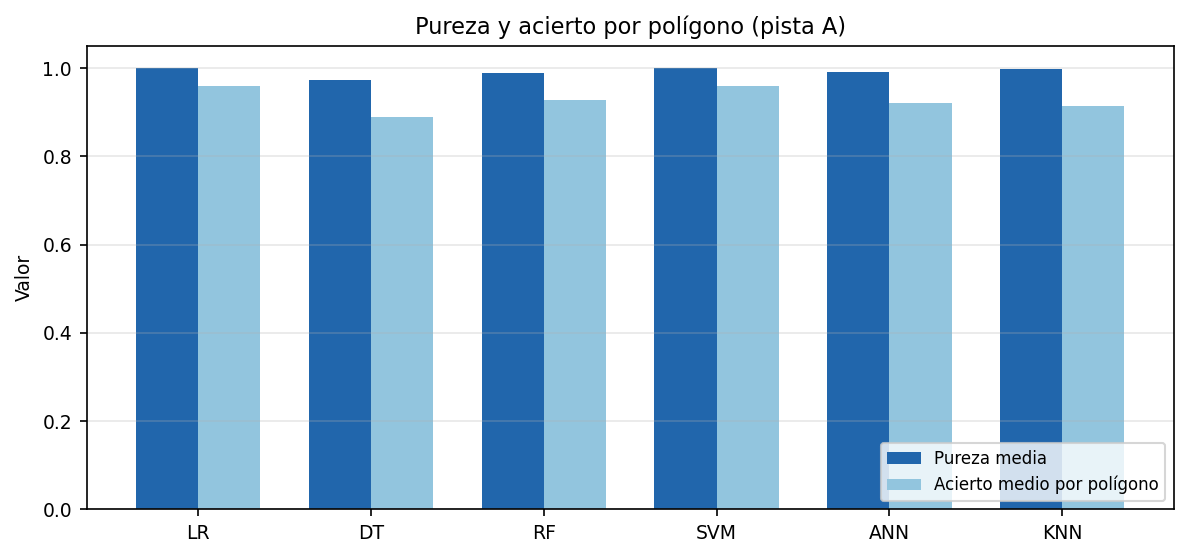
\includegraphics[width=0.85\textwidth]{figures/pureza_poligonos}
 \caption{Pureza media y acierto medio por polígono de la pista A.}
 \label{fig:pureza}
\end{figure}

\subsection{Comparación píxel vs polígono}
La Tabla~\ref{tab:pixel_vs_poligono} y la Figura~\ref{fig:pixel_vs_poligono} comparan las tres evaluaciones. Al pasar de píxel a polígono, la OA de la regresión logística sube de 0{,}947 a 0{,}958 y la de la SVM también sube de 0{,}947 a 0{,}958. La evaluación por polígono es más estable porque evita que unos pocos píxeles mezclados dominen la métrica, pero también es más gruesa: solo hay 24 polígonos de prueba.

\begin{table}[htbp]
 \centering
 \small
 \caption{Comparación de la unidad de evaluación: píxel, polígono A (votación) y polígono B (medianas).}
 \label{tab:pixel_vs_poligono}
 \begin{tabular}{lcccccc}
  \toprule
  Modelo & OA píxel & Kappa píxel & OA pol. A & Kappa pol. A & OA pol. B & Kappa pol. B \\
  \midrule
  LR & 0{,}947 & 0{,}935 & 0{,}958 & 0{,}950 & 0{,}958 & 0{,}950 \\
  DT & 0{,}867 & 0{,}837 & 0{,}917 & 0{,}900 & 0{,}917 & 0{,}900 \\
  RF & 0{,}909 & 0{,}888 & 0{,}917 & 0{,}900 & 0{,}958 & 0{,}950 \\
  SVM & 0{,}947 & 0{,}935 & 0{,}958 & 0{,}950 & 0{,}917 & 0{,}900 \\
  ANN & 0{,}898 & 0{,}875 & 0{,}917 & 0{,}900 & 0{,}917 & 0{,}900 \\
  KNN & 0{,}892 & 0{,}868 & 0{,}917 & 0{,}900 & 0{,}875 & 0{,}850 \\
  \bottomrule
 \end{tabular}
\end{table}


\begin{figure}[htbp]
 \centering
 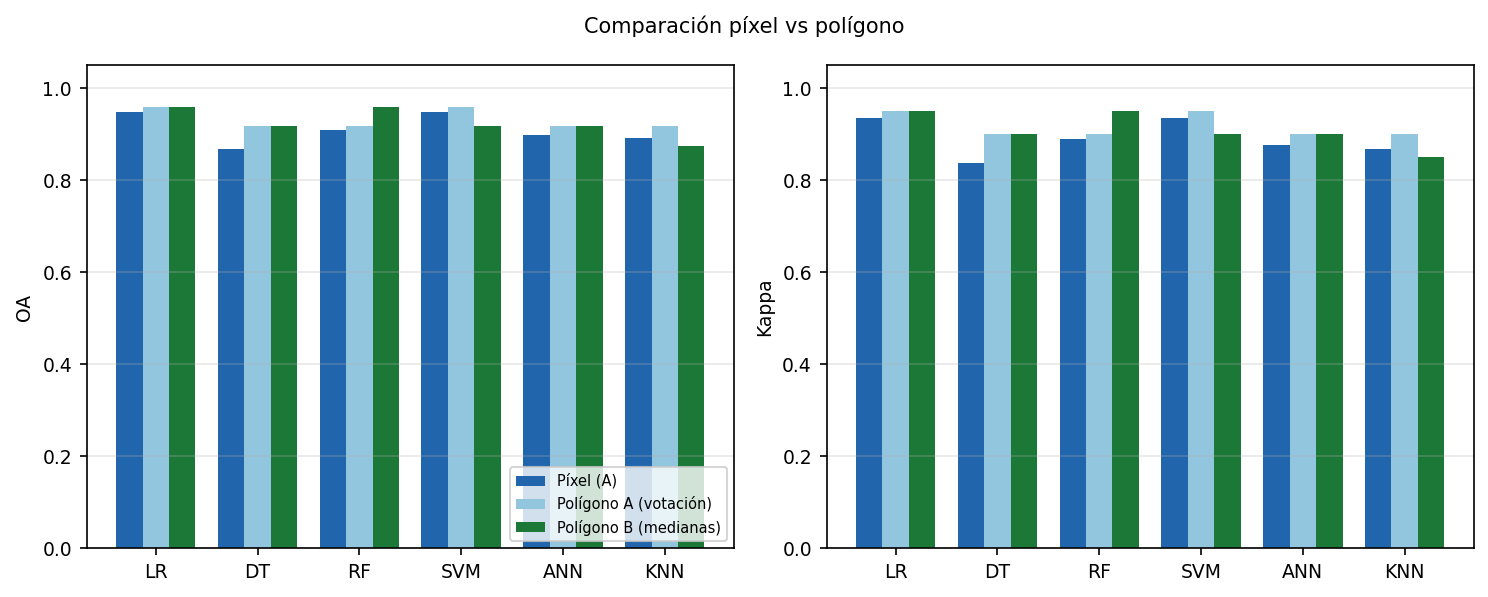
\includegraphics[width=0.95\textwidth]{figures/pixel_vs_poligono}
 \caption{OA y Kappa según la unidad de evaluación: píxel, polígono A (votación) y polígono B (medianas).}
 \label{fig:pixel_vs_poligono}
\end{figure}

\subsection{Unidad de muestreo y tamaño efectivo}
La Tabla~\ref{tab:icc} presenta la correlación intraclase (ICC) por banda y el tamaño efectivo de muestra. El ICC es 0{,}932--0{,}995 y el tamaño efectivo es 88--94, no 1640. Es decir, los píxeles de un mismo polígono aportan muy poca información independiente. Esto justifica partir y evaluar por polígono, y explica por qué añadir píxeles dentro de los polígonos existentes no equivale a añadir datos.

\begin{table}[htbp]
 \centering
 \small
 \caption{Correlación intraclase (ICC) por banda y tamaño efectivo de muestra considerando el polígono como unidad.}
 \label{tab:icc}
 \begin{tabular}{lcc}
  \toprule
  Banda & ICC & $n_{\mathrm{eff}}$ \\
  \midrule
  B01 & 0{,}993 & 88{,}6 \\
  B02 & 0{,}932 & 94{,}0 \\
  B03 & 0{,}949 & 92{,}5 \\
  B04 & 0{,}968 & 90{,}7 \\
  B05 & 0{,}980 & 89{,}7 \\
  B06 & 0{,}984 & 89{,}3 \\
  B07 & 0{,}986 & 89{,}2 \\
  B08 & 0{,}975 & 90{,}2 \\
  B8A & 0{,}991 & 88{,}8 \\
  B09 & 0{,}995 & 88{,}4 \\
  B11 & 0{,}988 & 89{,}1 \\
  B12 & 0{,}988 & 89{,}0 \\
  \bottomrule
 \end{tabular}
\end{table}


\subsection{Importancia de las variables}
La Figura~\ref{fig:importancia} muestra la importancia de las bandas en la pista A. El árbol de decisión se apoya en B8A, B12 y B02; el Random Forest reparte la importancia entre B8A, B12 y B04. La Figura~\ref{fig:importancia_pol} muestra la pista B: NDVI, NDWI y MNDWI concentran la mayor importancia, seguidas de B03, B07 y B12. Esta importancia debe leerse con cuidado: NDVI, NDWI y MNDWI son los mismos índices con los que se propusieron las etiquetas, así que su peso está inflado por construcción y no demuestra que aporten información nueva.

\begin{figure}[htbp]
 \centering
 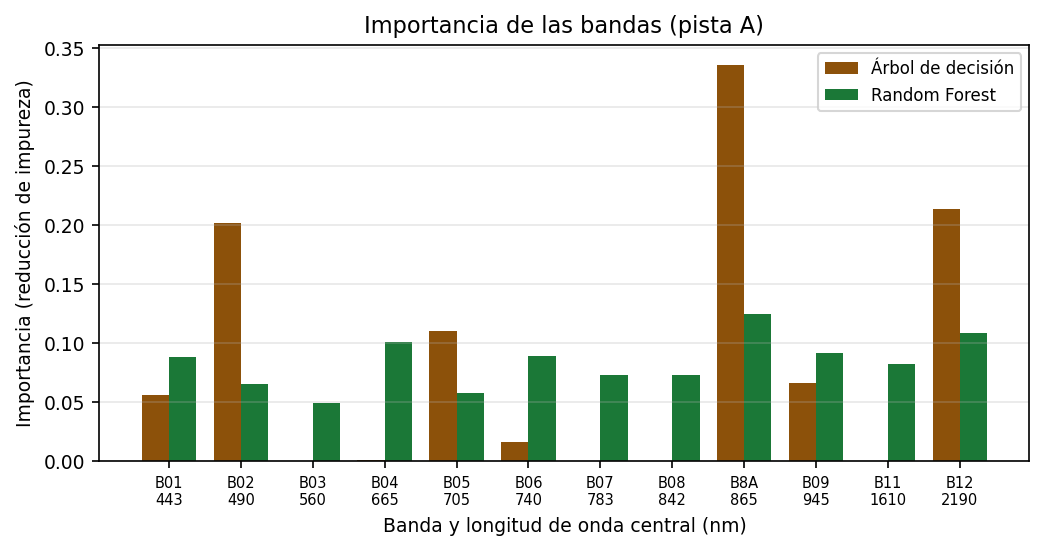
\includegraphics[width=0.85\textwidth]{figures/importancia_bandas}
 \caption{Importancia de las bandas (reducción media de la impureza de Gini) en el árbol de decisión y el Random Forest de la pista A.}
 \label{fig:importancia}
\end{figure}

\begin{figure}[htbp]
 \centering
 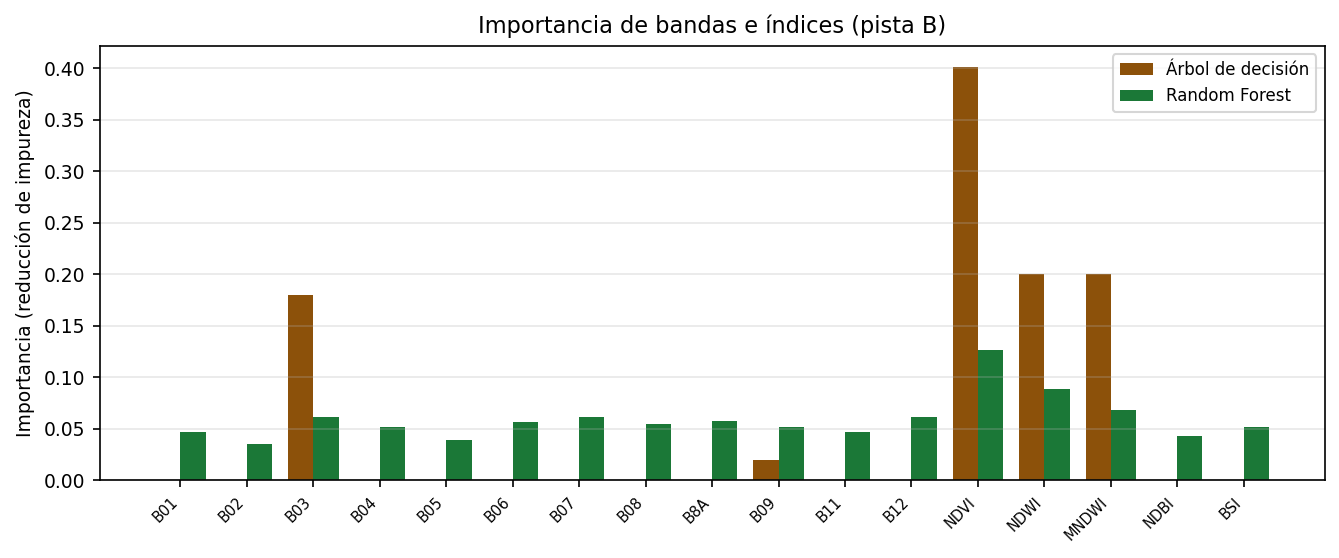
\includegraphics[width=0.95\textwidth]{figures/importancia_bandas_poligono}
 \caption{Importancia de bandas e índices en el árbol de decisión y el Random Forest de la pista B.}
 \label{fig:importancia_pol}
\end{figure}

\section{Discusión}
Los resultados indican que las doce bandas permiten separar con exactitud la vegetación, el agua y el relave. La dificultad está en suelo expuesto y urbano: sus firmas son parecidas y, a 10\,m, un polígono de suelo puede contener lotes, vías o materiales de construcción. El error de \texttt{5\_06} es consistente con esa ambigüedad: no es un píxel aislado, es un polígono completo.

La ampliación del dataset no mejoró de forma demostrable el desempeño. Se retiraron dos polígonos de suelo después de ver que la SVM los fallaba y se añadieron candidatos de suelo, agua y urbano al entrenamiento. Sobre la prueba original la SVM se mantiene en 89{,}4\,\% y la regresión logística sube 1{,}1 puntos, hasta 89{,}4\,\%. El 94{,}7\,\% de la prueba actual describe un conjunto sin los dos polígonos difíciles, no una mejora de los modelos. La red neuronal queda en 0{,}898 en la prueba actual, por debajo de los modelos más simples.

Quedan limitaciones. Las etiquetas son pseudo-etiquetas construidas con reglas espectrales y revisión visual, no verdad de campo. Cinco polígonos añadidos quedaron a 10--60\,m de polígonos de prueba, por debajo de la separación mínima de la Fase~1; aunque se comprobó que no cambian la exactitud, introducen autocorrelación espacial. Los 72 polígonos originales y los candidatos de suelo no tuvieron revisión visual individual. El test tiene solo 24 polígonos y las clases de vegetación y relave siguen con 12 polígonos cada una. Por eso las diferencias de uno o dos polígonos no deben interpretarse como superioridad definitiva.

\part{Fase 3: optimización, predicción y análisis}
\label{part:fase3}

\section{Contexto y objetivos}

La Fase~1 definió el evento, el área de estudio y la escena Sentinel-2 del 1 de febrero de 2019. La Fase~2 documentó el archivo \texttt{training\_dataset.tsv}, entrenó cinco modelos del enunciado más Random Forest y reportó las métricas iniciales. La Fase~3 tiene tres objetivos:

\begin{enumerate}
 \item optimizar los hiperparámetros de cada arquitectura con validación agrupada por polígono;
 \item seleccionar un modelo con un criterio fijado antes de mirar el test y evaluarlo una sola vez;
 \item aplicar el modelo a toda la imagen, generar el GeoTIFF temático, simbolizarlo en QGIS y cuantificar el área de cada clase.
\end{enumerate}

\section{Datos y protocolo}

El conjunto de entrenamiento contiene 1640 píxeles de 10\,m distribuidos en 88 polígonos y seis clases: vegetación densa, vegetación baja, agua, relave minero, suelo expuesto y urbano. La división de la Fase~2 se mantuvo sin cambios: 64 polígonos y 1168 píxeles para entrenamiento, 24 polígonos y 472 píxeles para prueba. Ningún polígono aparece en ambos conjuntos.

La Fase~3 no amplió ni reetiquetó el dataset. En particular, el polígono de suelo \texttt{5\_06}, que el modelo de la Fase~2 clasifica completo como urbano, se conserva en el test para no favorecer al modelo. La comparación con la versión de 72 polígonos se documenta por separado en \texttt{report\_fase2}; la prueba actual no es pareada con la anterior.

Se usó la pista oficial por píxel con las doce bandas espectrales. La pista B, basada en medianas por polígono, se conserva como análisis exploratorio de la Fase~2 y no se usa para el mapa final.

\section{Optimización de hiperparámetros}

\subsection{Protocolo}

La búsqueda se hizo solo con los 64 polígonos de entrenamiento, mediante \texttt{StratifiedGroupKFold} de cuatro pliegues con semilla 42 \parencite{Roberts2017}. La métrica de selección fue el Kappa medio; se registraron también F1 macro y exactitud balanceada. El test congelado no participó en la búsqueda ni en la selección.

Se evaluaron 224 combinaciones: 10 de regresión logística, 80 de árbol de decisión, 30 de Random Forest, 50 de SVM, 30 de red neuronal y 24 de KNN. Los espacios fueron:

\begin{itemize}
 \item LR: $C \in \{0{,}01, 0{,}1, 1, 10, 100\}$ y pesos \texttt{None}/\texttt{balanced};
 \item DT: profundidad, hojas mínimas, criterio y pesos;
 \item RF: 300/500 árboles, profundidad, hojas mínimas, variables por división y pesos balanceados;
 \item SVM: $C$, $\gamma$ y pesos;
 \item ANN: arquitectura, $\alpha$ y tasa de aprendizaje;
 \item KNN: $k$, pesos y distancia.
\end{itemize}

Los modelos se estandarizaron dentro de un \texttt{Pipeline} ajustado solo con cada pliegue de entrenamiento. Para evitar que un candidato con alta varianza entre pliegues se impusiera por una diferencia pequeña, se aplicó una regla de una desviación estándar: dentro de la familia ganadora se consideraron los candidatos con Kappa a menos de un error estándar del mejor; entre ellos se prefirieron los pesos balanceados y la menor desviación entre pliegues.

\subsection{Resultados de la búsqueda}

\begin{table}[htbp]
 \centering
 \small
 \setlength{\tabcolsep}{4pt}
 \caption{Mejor Kappa de validación agrupada por familia. La columna final marca la familia seleccionada.}
 \label{tab:hpo}
 \begin{tabular}{lcccc}
  \toprule
  Modelo & Kappa CV & F1 CV & Candidatos & Seleccionado \\
  \midrule
  LR & 0{,}938 & 0{,}956 & 10 & Sí \\
  SVM & 0{,}918 & 0{,}938 & 50 & No \\
  ANN & 0{,}915 & 0{,}938 & 30 & No \\
  KNN & 0{,}904 & 0{,}931 & 24 & No \\
  RF & 0{,}856 & 0{,}895 & 30 & No \\
  DT & 0{,}791 & 0{,}829 & 80 & No \\
  \bottomrule
 \end{tabular}
\end{table}


La regresión logística tuvo el mejor Kappa medio (0{,}938), seguida por SVM (0{,}918), ANN (0{,}915), KNN (0{,}904), RF (0{,}856) y DT (0{,}791). La diferencia entre LR y SVM es de dos puntos porcentuales, pero la desviación entre pliegues también es apreciable y el test tiene solo 24 polígonos.

El mejor candidato de LR fue $C=100$ sin pesos balanceados, con Kappa 0{,}938 y una desviación de 0{,}066. Ese candidato tiene un Kappa de entrenamiento de 1{,}000 y una alta varianza; no se consideró una base estable. Dentro de una desviación estándar, la configuración $C=1$ con \texttt{class\_weight=balanced} quedó entre las más estables (Kappa 0{,}892, desviación 0{,}044) y fue la elegida. La Tabla~\ref{tab:params_finales} resume sus parámetros.

\begin{table}[htbp]
 \centering
 \small
 \setlength{\tabcolsep}{4pt}
 \caption{Hiperparámetros del modelo final (Regresión logística).}
 \label{tab:params_finales}
 \begin{tabular}{ll}
  \toprule
  Parámetro & Valor \\
  \midrule
  C & 1.0 \\
  class\_weight & balanced \\
  \bottomrule
 \end{tabular}
\end{table}


\begin{figure}[htbp]
 \centering
 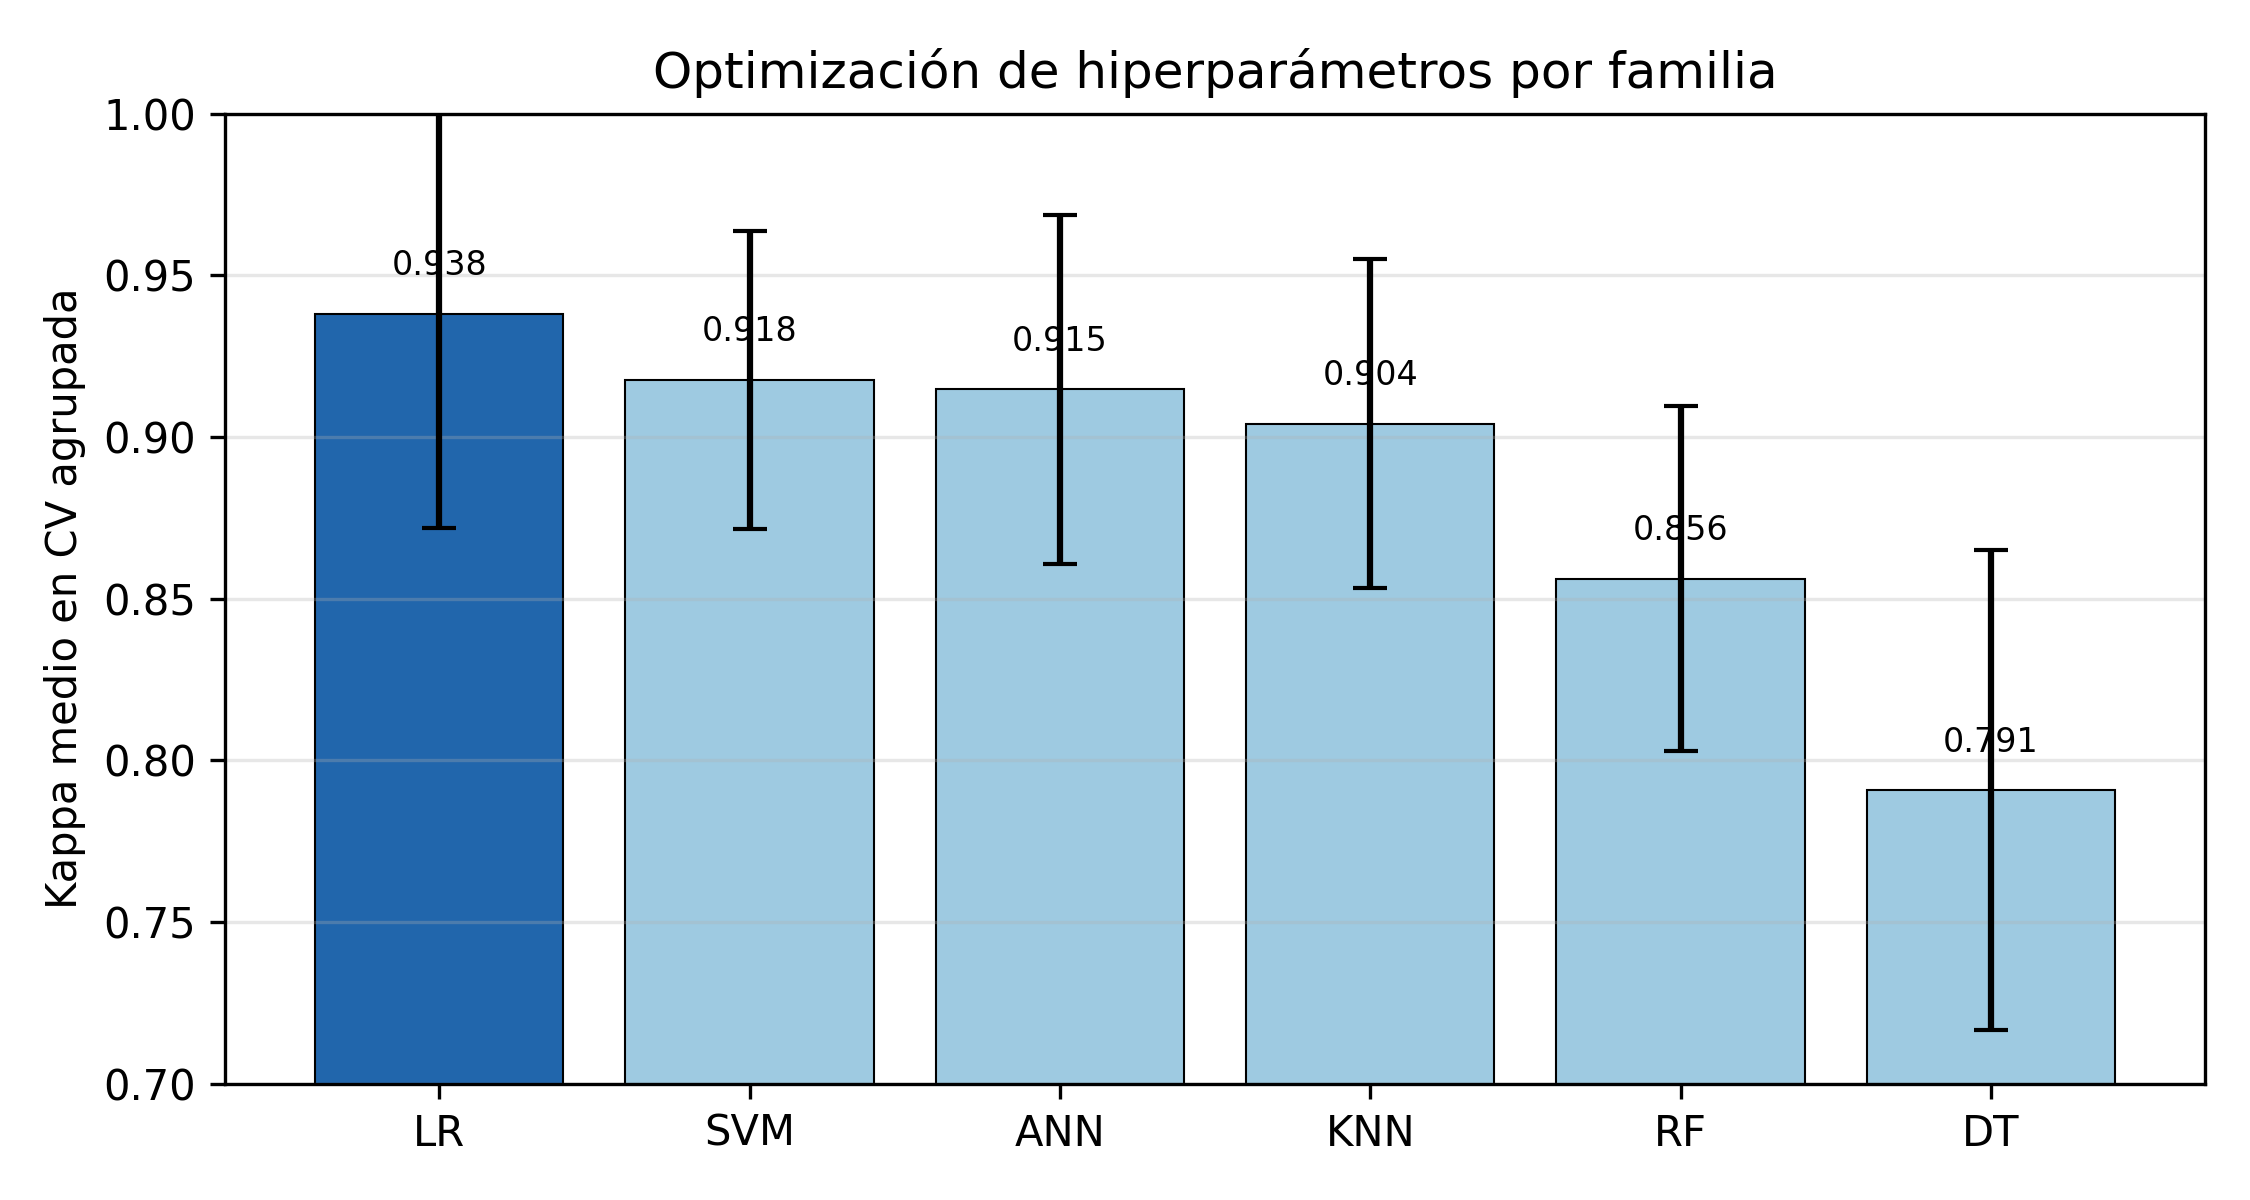
\includegraphics[width=0.82\textwidth]{figures/fase3_hpo_modelos}
 \caption{Kappa medio de la mejor configuración de cada familia en la validación agrupada. Las barras de error son la desviación estándar entre pliegues.}
 \label{fig:f3_hpo}
\end{figure}

\section{Evaluación en el test congelado}

Los seis modelos tuneados se entrenaron con los 64 polígonos de entrenamiento y se evaluaron una sola vez en los 24 polígonos de prueba. La Tabla~\ref{tab:phase3_metricas} y la Figura~\ref{fig:f3_tuned} resumen los resultados.

\begin{table}[htbp]
 \centering
 \small
 \setlength{\tabcolsep}{4pt}
 \caption{Métricas en el test congelado de 24 polígonos y Kappa de validación agrupada. \emph{CV familia} es el mejor Kappa de la familia; \emph{CV modelo} es el del conjunto de hiperparámetros elegido.}
 \label{tab:phase3_metricas}
 \begin{tabular}{lcccccc}
  \toprule
  Modelo & OA & Kappa & F1 & CV modelo & CV familia & Final \\
  \midrule
  LR & 0{,}947 & 0{,}935 & 0{,}933 & 0{,}892 & 0{,}938 & Sí \\
  RF & 0{,}917 & 0{,}899 & 0{,}910 & 0{,}856 & 0{,}856 & No \\
  ANN & 0{,}911 & 0{,}891 & 0{,}905 & 0{,}915 & 0{,}915 & No \\
  SVM & 0{,}890 & 0{,}865 & 0{,}888 & 0{,}918 & 0{,}918 & No \\
  KNN & 0{,}890 & 0{,}865 & 0{,}886 & 0{,}904 & 0{,}904 & No \\
  DT & 0{,}864 & 0{,}835 & 0{,}847 & 0{,}791 & 0{,}791 & No \\
  \bottomrule
 \end{tabular}
\end{table}


La regresión logística obtuvo la mejor exactitud global (0{,}947), el mejor Kappa (0{,}935) y el mejor F1 macro (0{,}933). Random Forest quedó en 0{,}917/0{,}899, la ANN en 0{,}911/0{,}891, SVM y KNN en 0{,}890/0{,}865, y el árbol de decisión en 0{,}864/0{,}835. La SVM, que en la Fase~2 empataba con LR, bajó al elegir un candidato con $C=100$; el resultado confirma que la búsqueda de hiperparámetros con 64 polígonos puede sobreajustar la validación.

\begin{figure}[htbp]
 \centering
 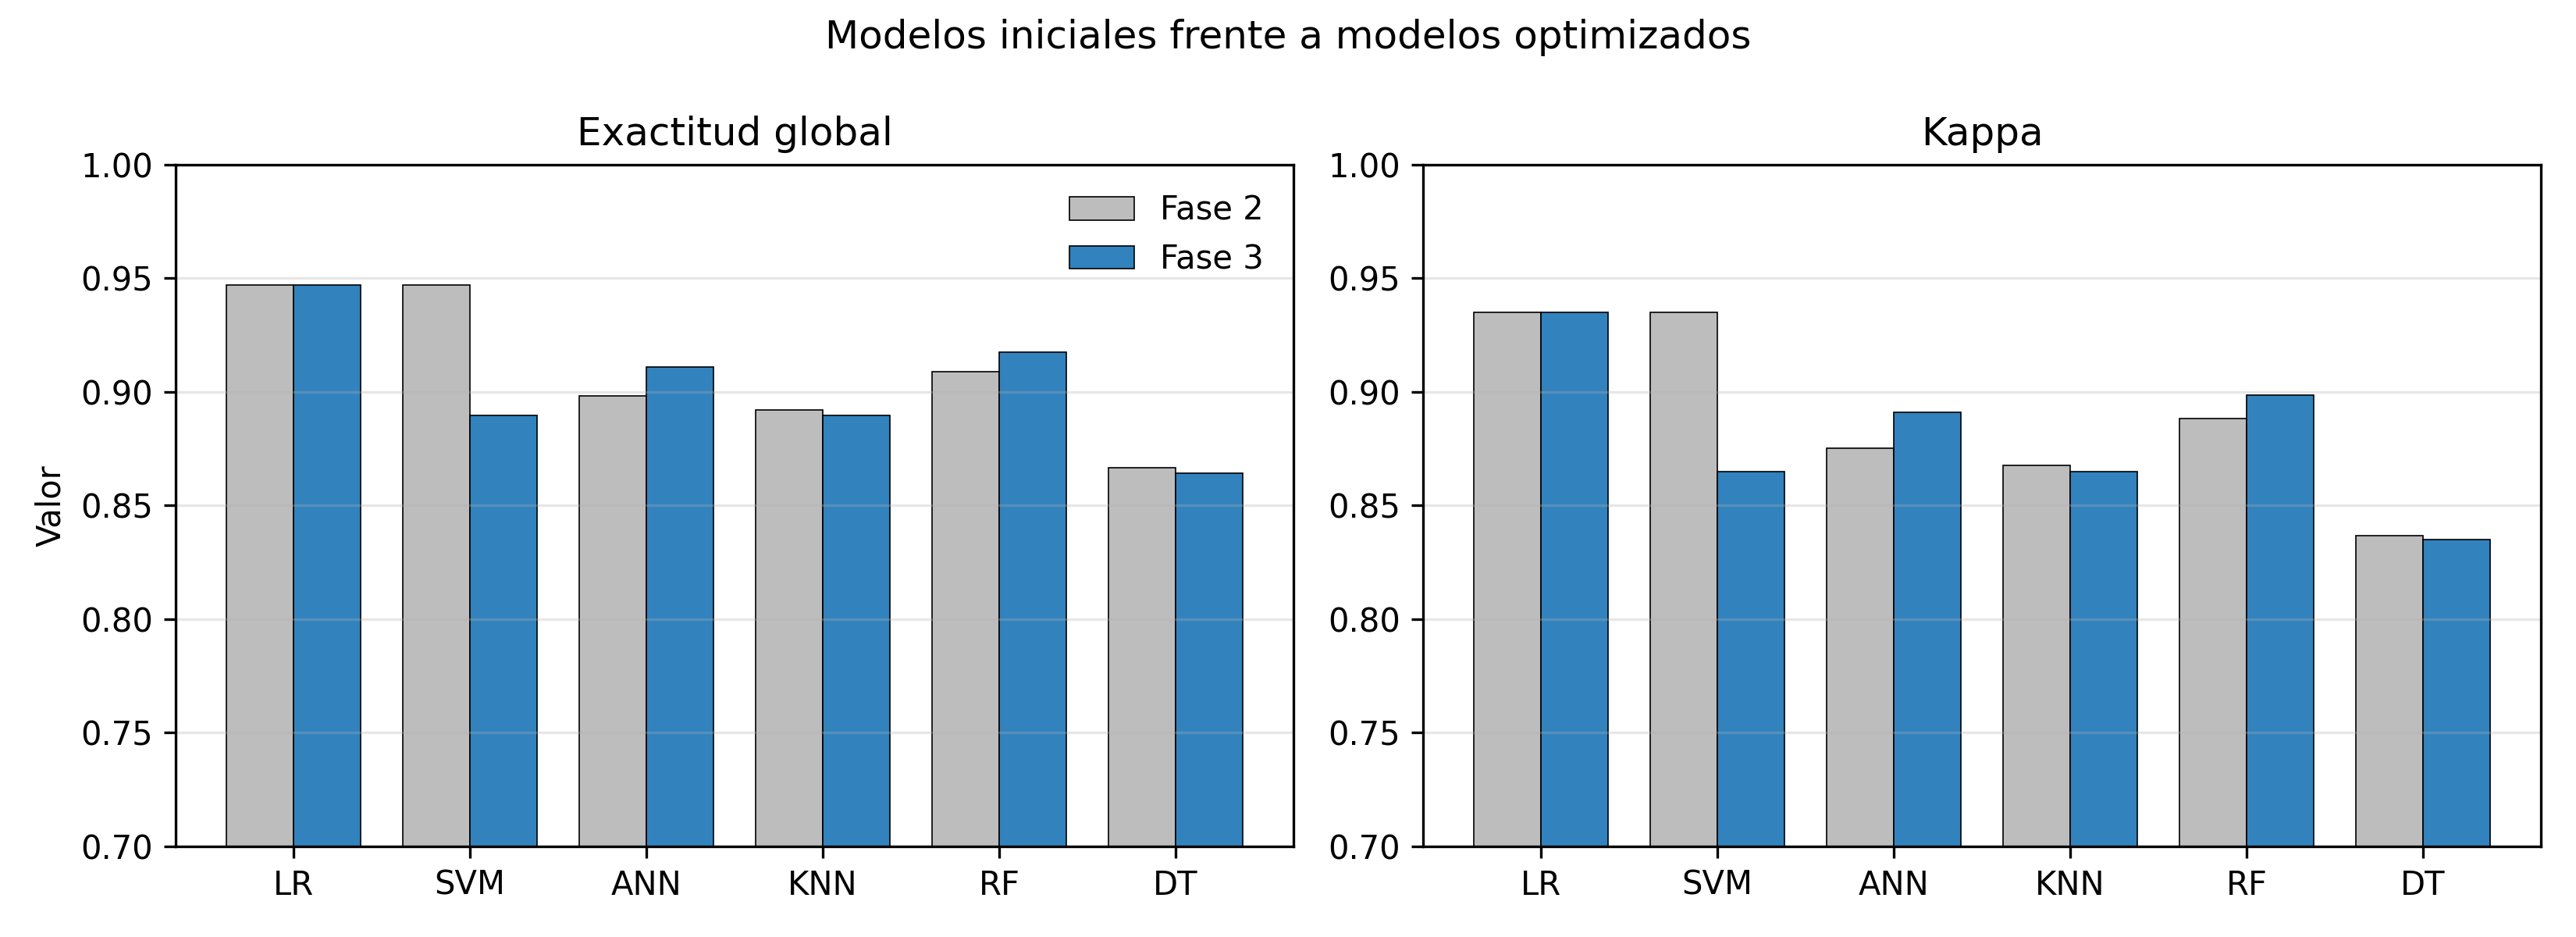
\includegraphics[width=\textwidth]{figures/fase3_tuned_vs_inicial}
 \caption{Exactitud global y Kappa de los modelos iniciales de la Fase~2 frente a los modelos optimizados de la Fase~3.}
 \label{fig:f3_tuned}
\end{figure}

El modelo final no mejora el resultado de la Fase~2: la regresión logística mantiene 0{,}947 de exactitud y 0{,}935 de Kappa. La conclusión de la Fase~3 no es que el HPO haya mejorado el clasificador, sino que la configuración regularizada de LR es la opción más estable dentro de un conjunto pequeño y muy correlacionado.

\subsection{Matriz de confusión e importancia}

La Figura~\ref{fig:f3_confusion} muestra la matriz de confusión del modelo final. Vegetación densa, vegetación baja, agua y relave se clasifican sin errores en el test. El único error es el polígono de suelo \texttt{5\_06}: sus 25 píxeles se asignan a urbano. Por eso el recall de suelo es 0{,}75 y la precisión de urbano es 0{,}59.

\begin{figure}[htbp]
 \centering
 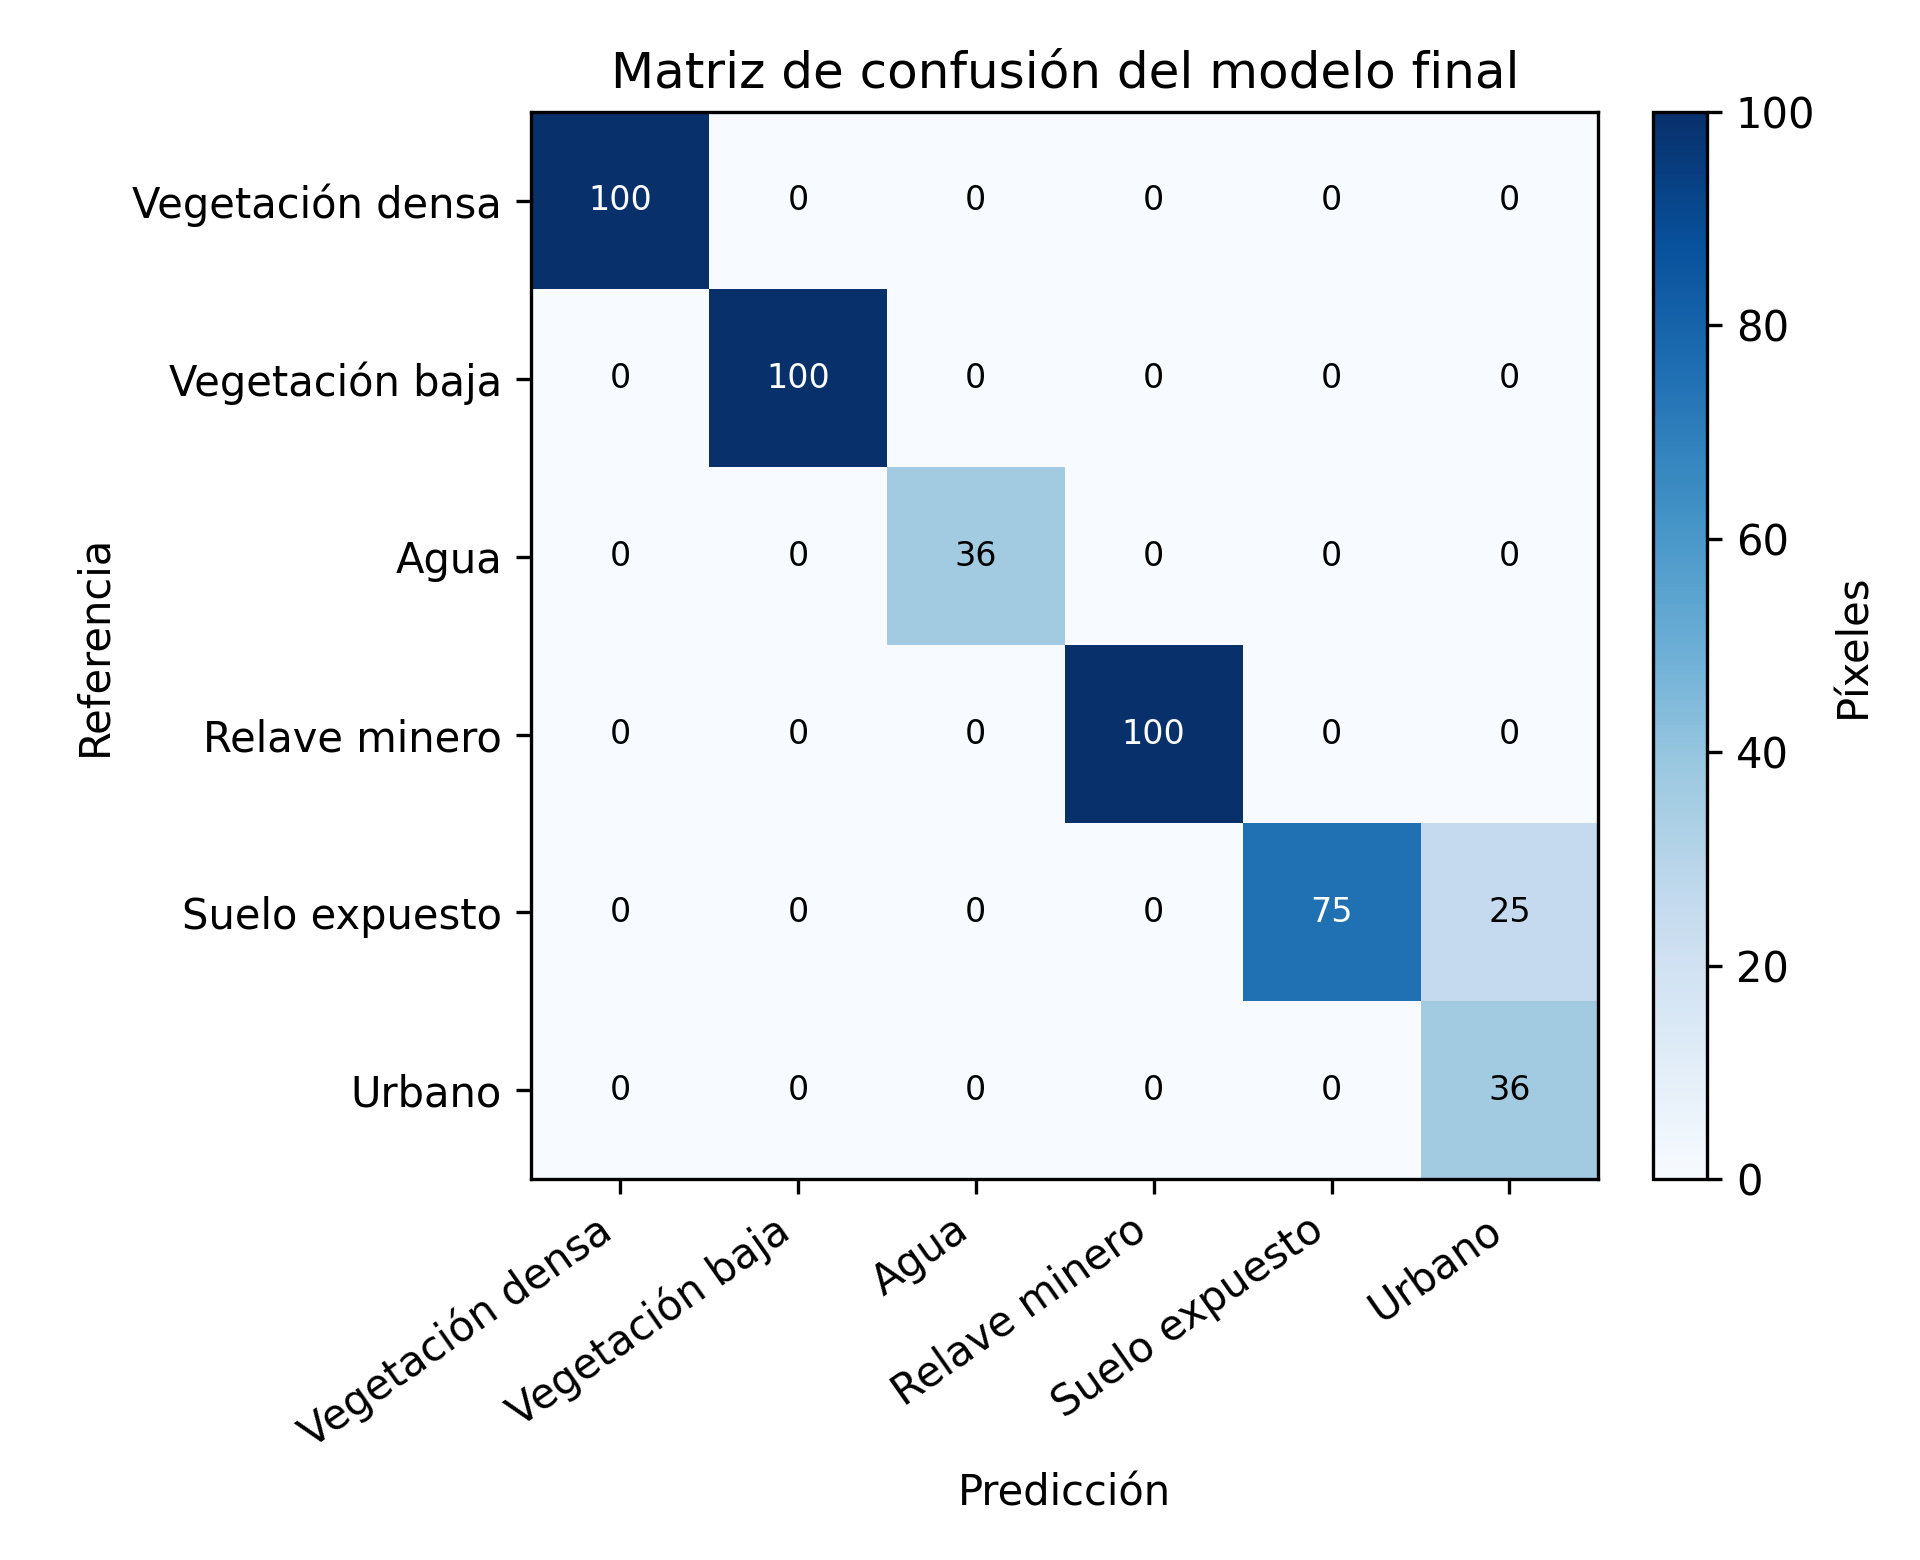
\includegraphics[width=0.72\textwidth]{figures/fase3_confusion_final}
 \caption{Matriz de confusión del modelo final sobre los 24 polígonos de prueba.}
 \label{fig:f3_confusion}
\end{figure}

La Figura~\ref{fig:f3_importance} presenta la importancia por permutación sobre el test. Las bandas B03, B09 y B02 concentran la mayor pérdida de exactitud al permutarse; B07, B8A y B08 aportan menos. Esta importancia es descriptiva: las bandas están correlacionadas y el test tiene 472 píxeles, por lo que no debe interpretarse como una prueba causal de la importancia espectral.

\begin{figure}[htbp]
 \centering
 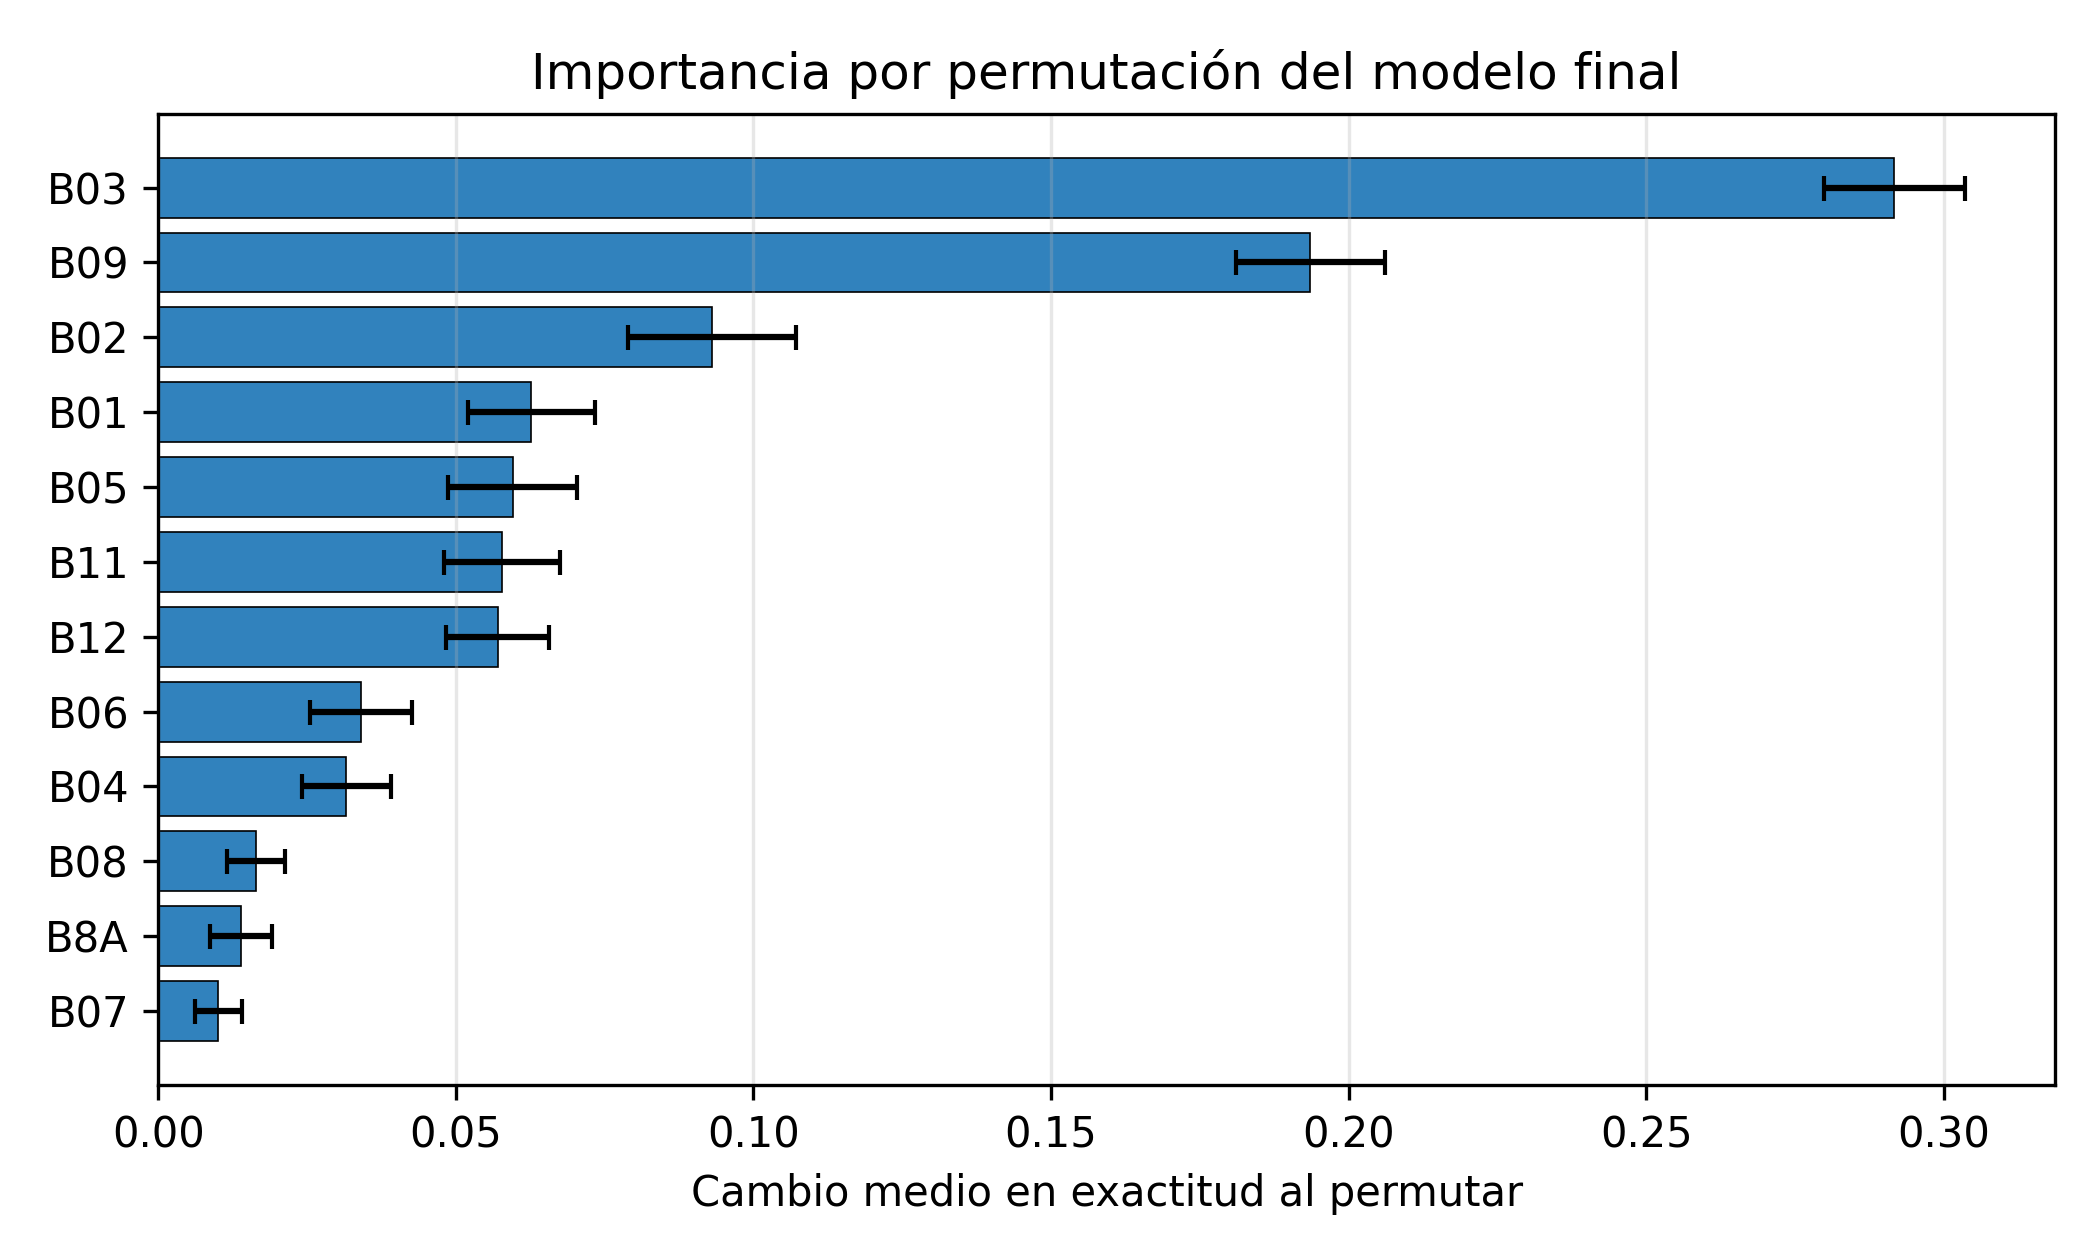
\includegraphics[width=0.8\textwidth]{figures/fase3_importancia_final}
 \caption{Importancia por permutación del modelo final. La barra es la media de 30 repeticiones y la línea el error estándar.}
 \label{fig:f3_importance}
\end{figure}

\subsection{Incertidumbre y estabilidad}

El intervalo bootstrap del 95\,\% para la exactitud global del modelo final es 0{,}841--1{,}000; para Kappa, 0{,}809--1{,}000; para F1 macro, 0{,}815--1{,}000. La amplitud refleja que cada polígono de prueba pesa aproximadamente 5{,}3 puntos porcentuales. En la validación dejando un polígono fuera, la exactitud media fue 0{,}946 con error estándar 0{,}024, y el Kappa out-of-fold fue 0{,}912. Las diferencias entre modelos no deben interpretarse como superioridad definitiva.

\section{Inferencia y GeoTIFF temático}

El modelo final se reentrenó con los 88 polígonos y se aplicó al stack de doce bandas. La inferencia se hizo por bloques de 128 filas para no cargar todo el ráster. Antes de predecir se enmascararon:

\begin{itemize}
 \item los píxeles fuera de \texttt{study\_area.gpkg};
 \item los píxeles con SCL inválida: 0, 1, 3, 8, 9 y 10;
 \item los píxeles sin datos del stack.
\end{itemize}

El resultado es un GeoTIFF de una banda, tipo \texttt{uint8}, con el mismo CRS (EPSG:32723), el mismo \emph{transform}, ancho y alto que la imagen original. El valor 0 representa “sin datos”; 1--6 son las clases. El archivo incluye una tabla de colores y se acompaña de un estilo QGIS \texttt{.qml}.

\begin{figure}[htbp]
 \centering
 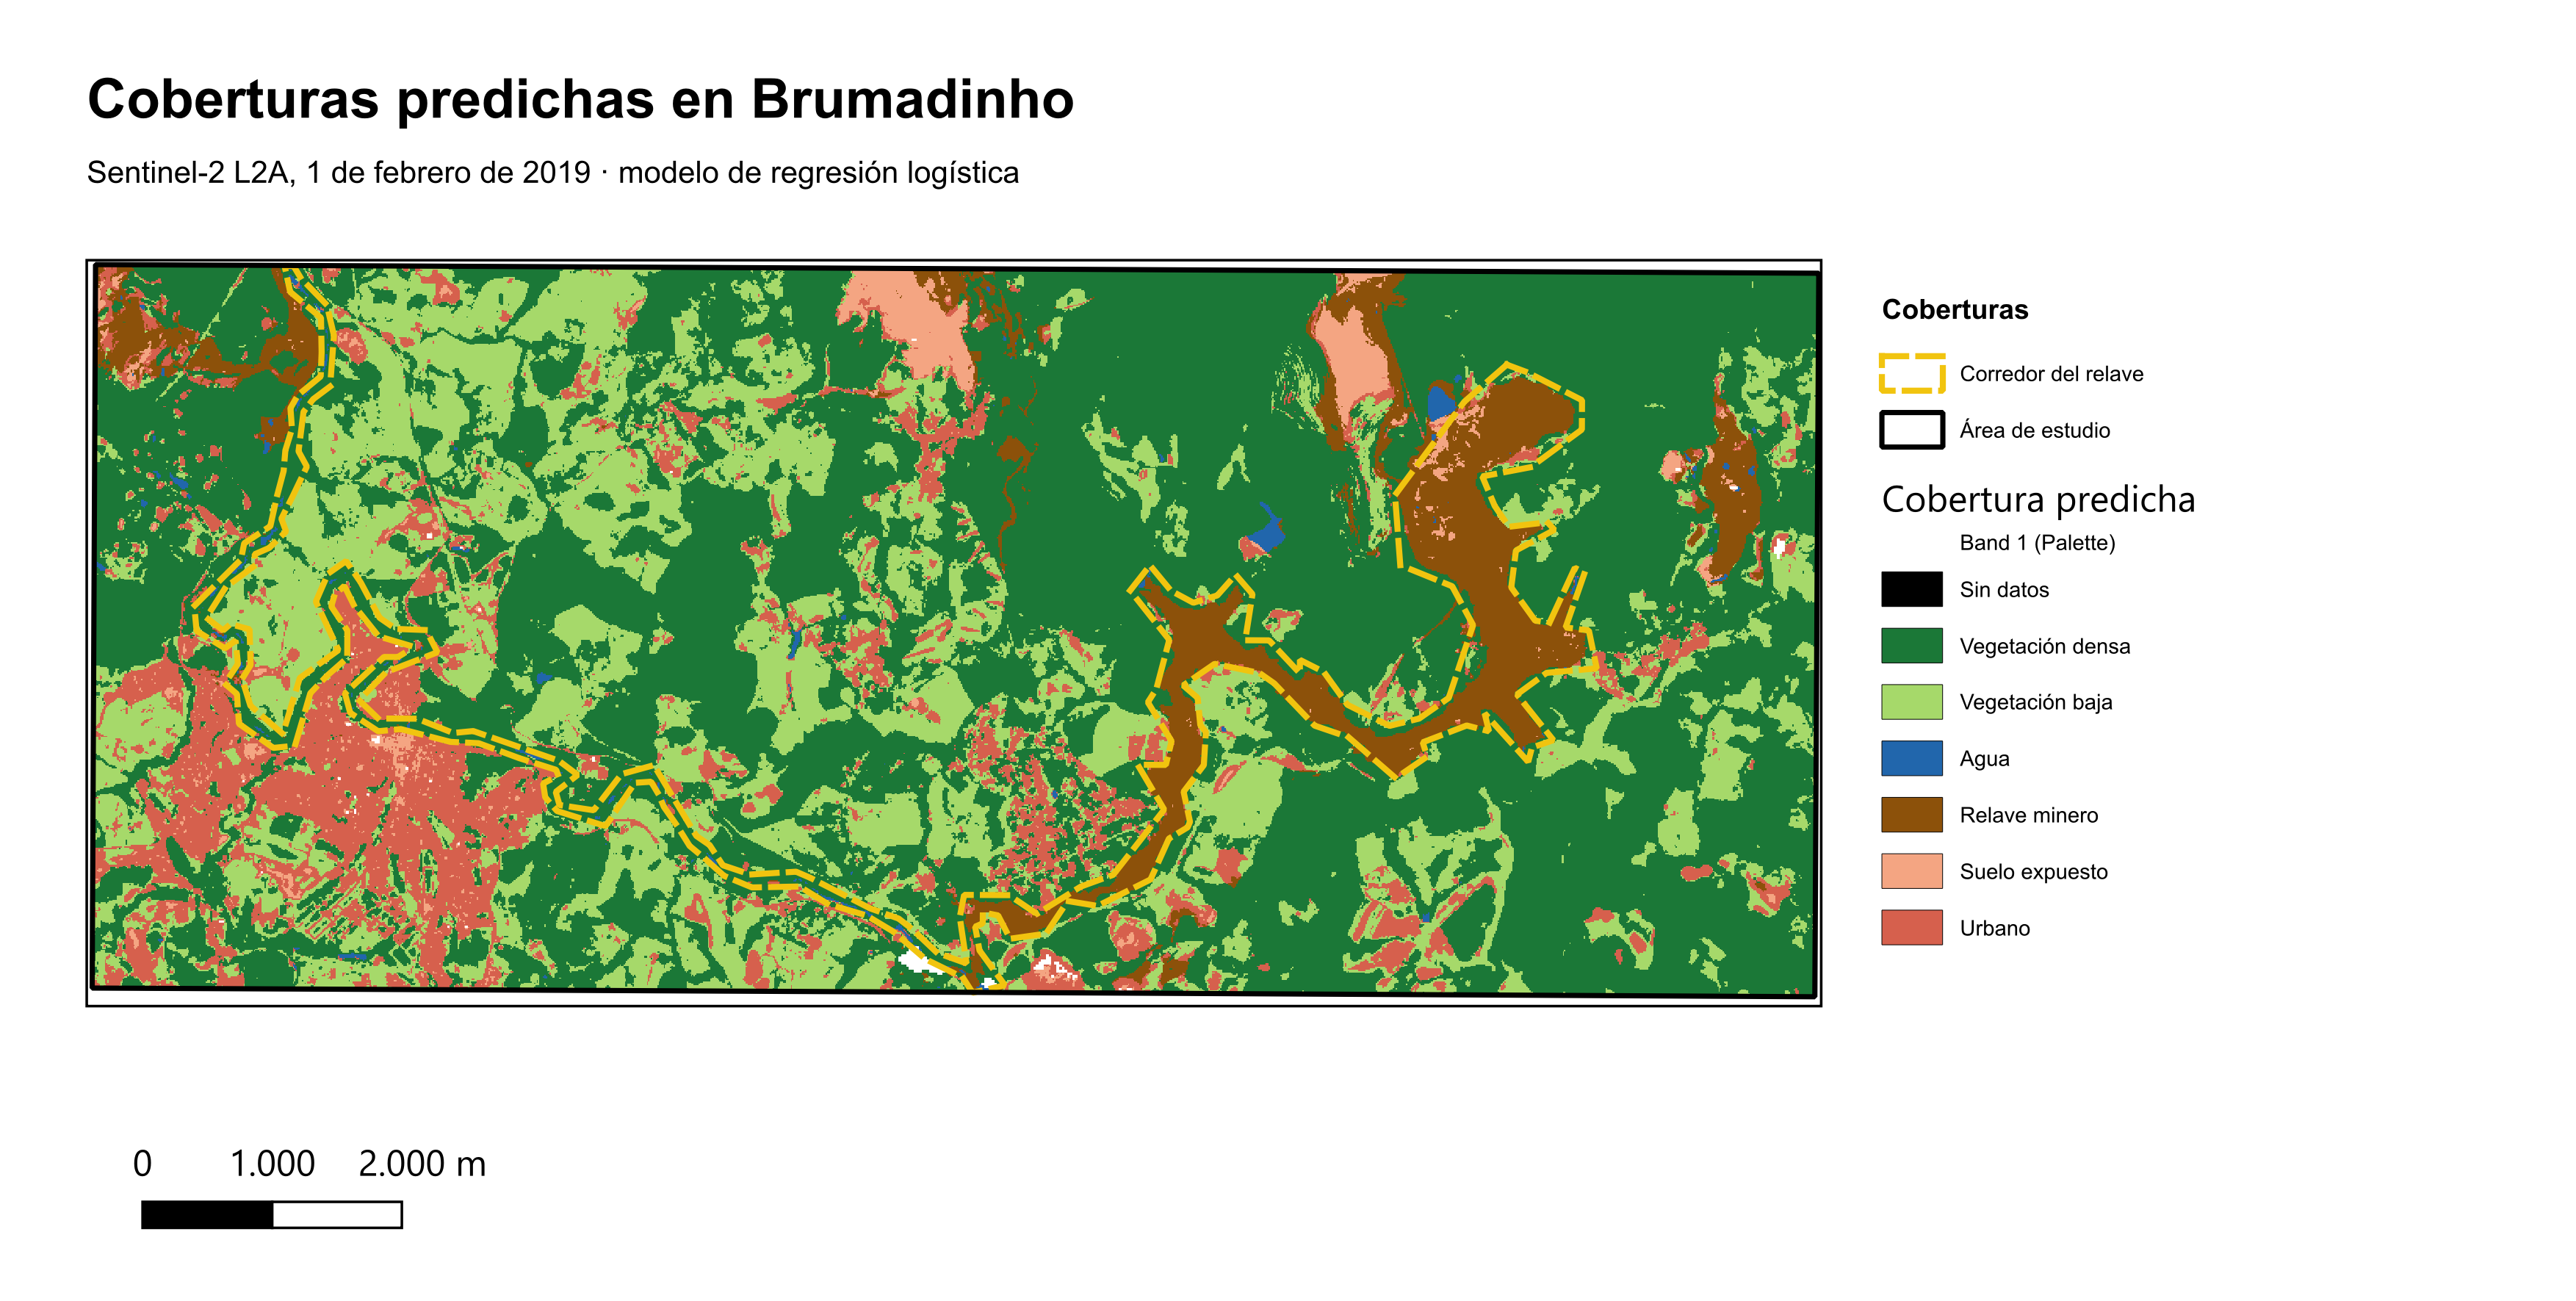
\includegraphics[width=\textwidth]{figures/fase3_mapa_tematico_qgis}
 \caption{Mapa temático exportado desde QGIS. El contorno negro delimita el área de estudio y la línea amarilla el corredor del relave.}
 \label{fig:f3_mapa}
\end{figure}

El mapa se generó con QGIS 4.2.2 a partir del GeoTIFF y del estilo discreto. La Figura~\ref{fig:f3_zoom} muestra el detalle del corredor del relave. La clase relave aparece a lo largo del corredor, pero también en zonas de la mina fuera de él; esa es una limitación de la separación espectral entre relave y suelo desnudo.

\begin{figure}[htbp]
 \centering
 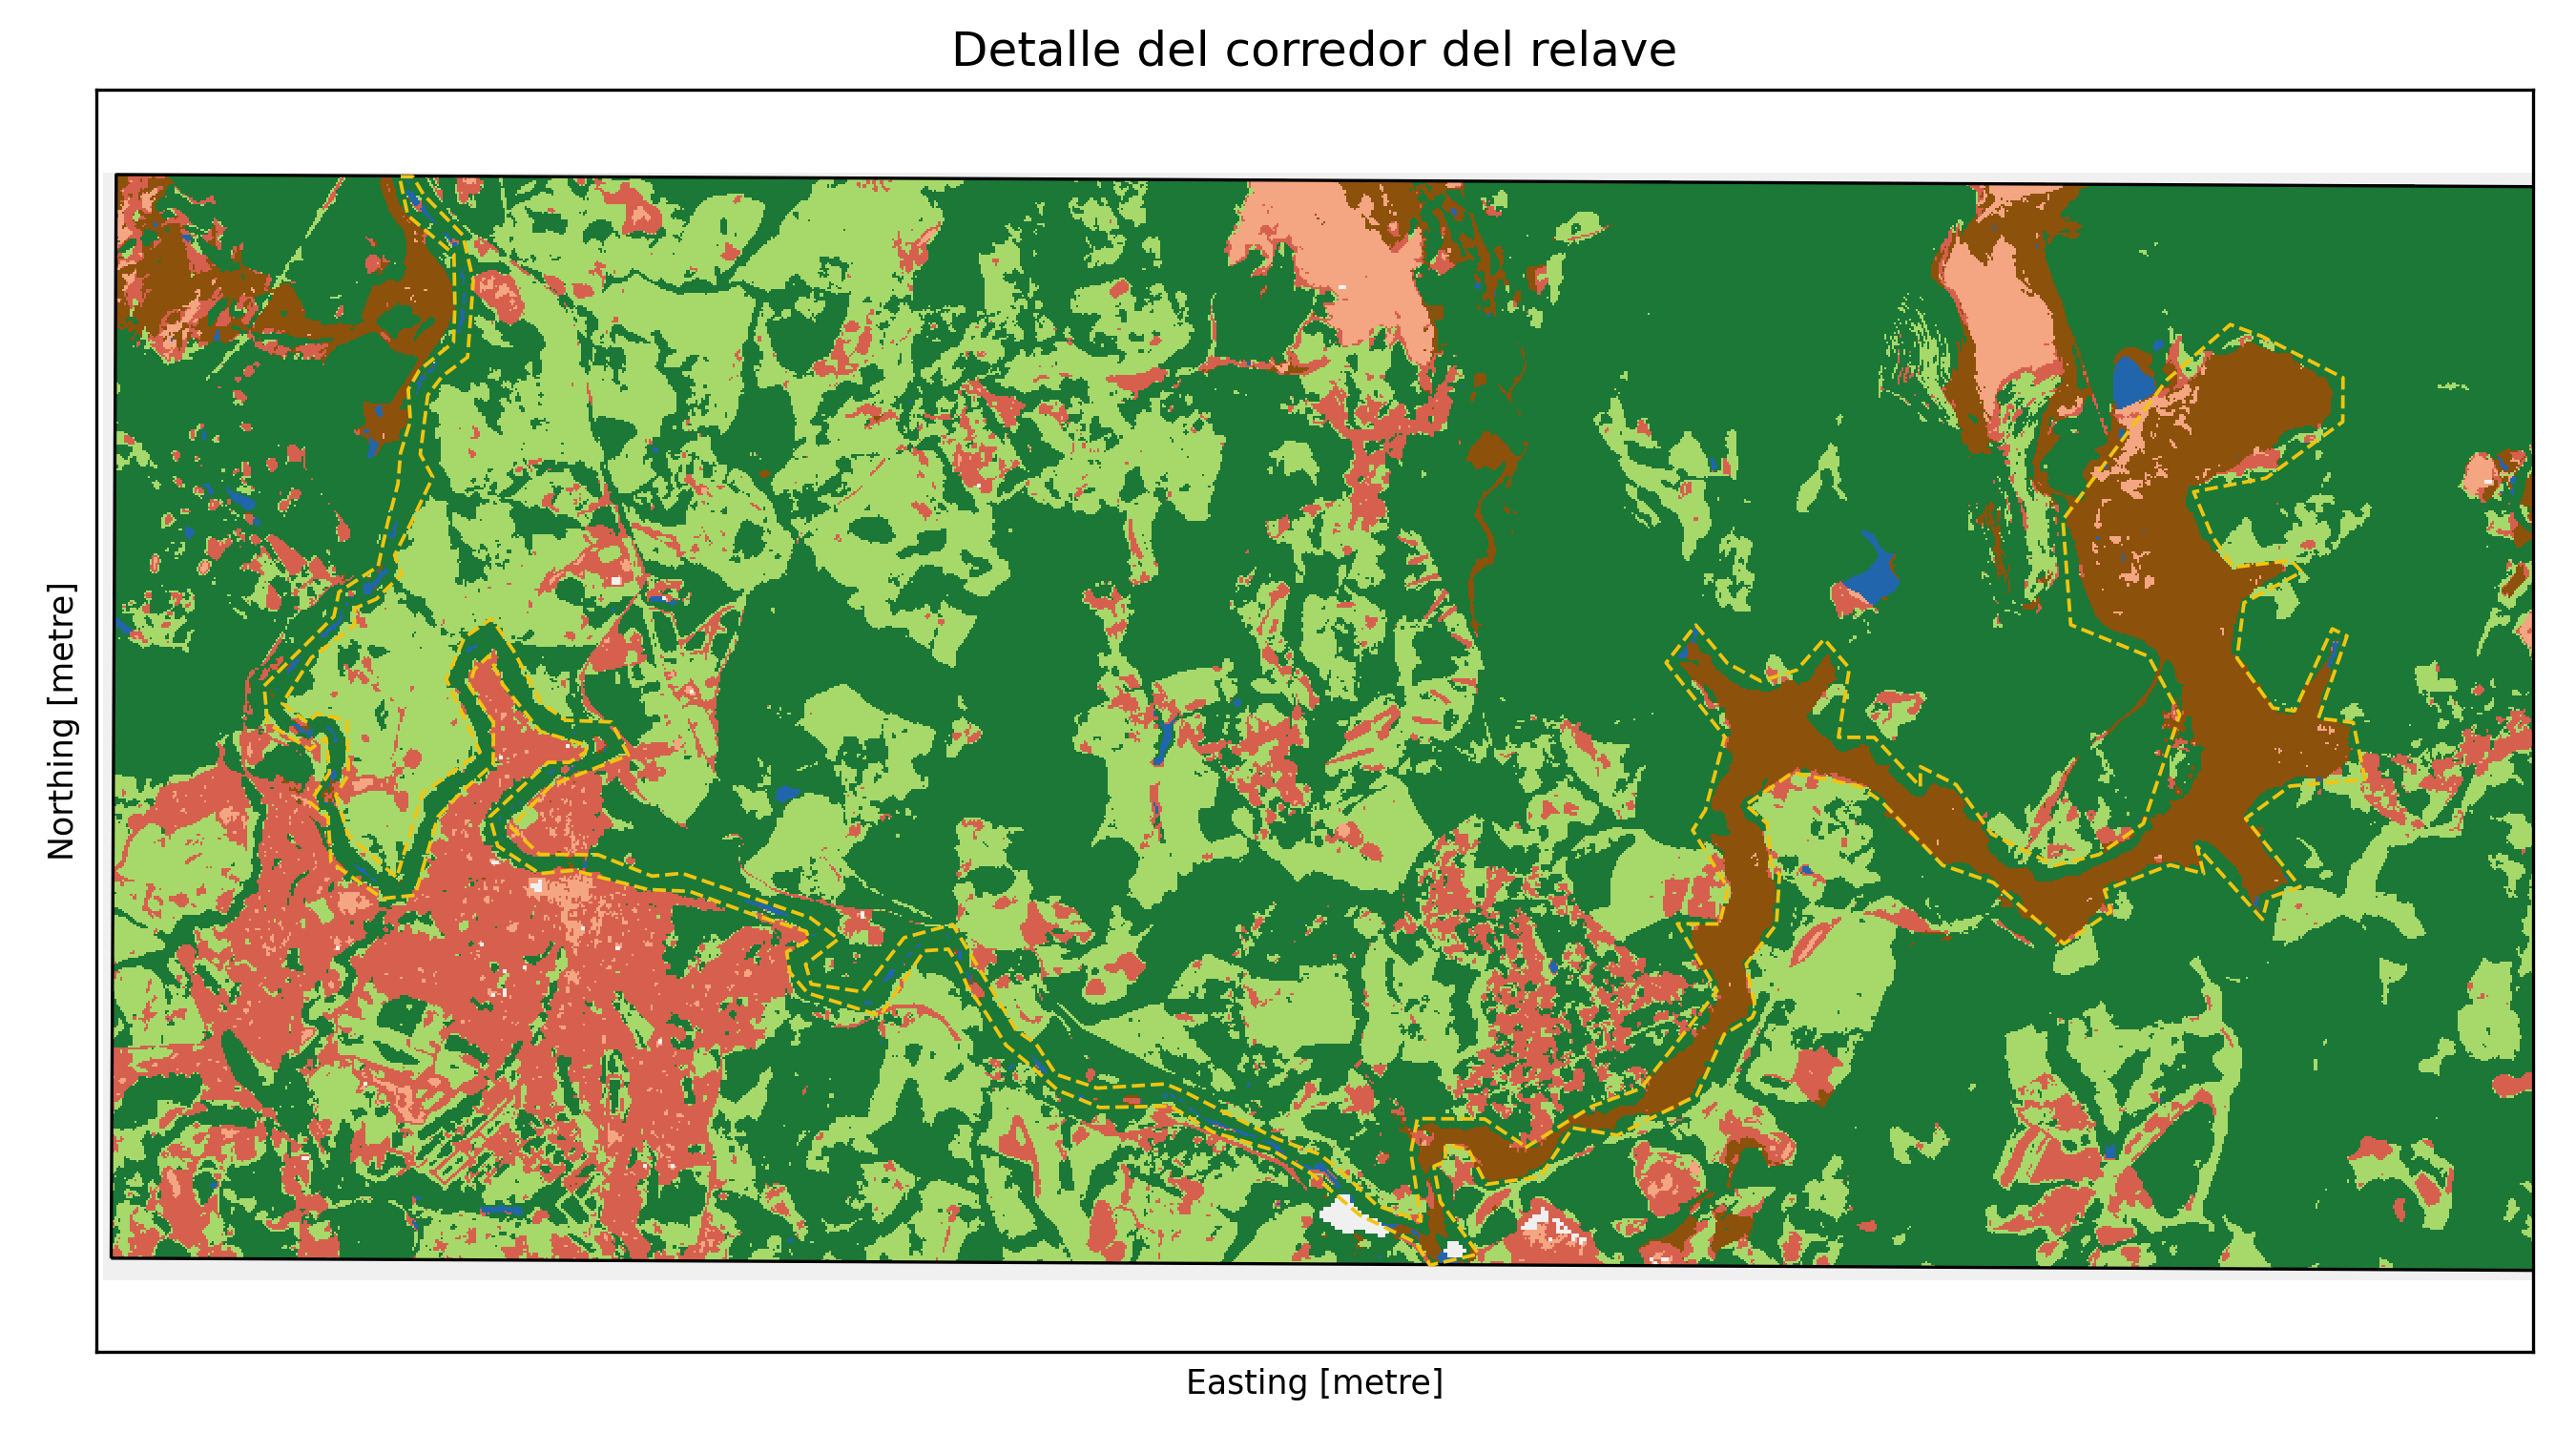
\includegraphics[width=0.9\textwidth]{figures/fase3_mapa_zoom_relave}
 \caption{Detalle del corredor del relave sobre el mapa predicho.}
 \label{fig:f3_zoom}
\end{figure}

\section{Cuantificación de áreas}

La Tabla~\ref{tab:area_clases} resume las áreas predichas. El área válida total es 74{,}100\,km$^2$; los 2{,}166\,km$^2$ restantes son “sin datos” e incluyen el exterior del polígono de estudio y los píxeles inválidos por SCL.

\begin{table}[htbp]
 \centering
 \small
 \setlength{\tabcolsep}{4pt}
 \caption{Área predicha por clase. Los porcentajes se calculan sobre el área válida, no sobre el rectángulo completo.}
 \label{tab:area_clases}
 \begin{tabular}{lcccc}
  \toprule
  Clase & Píxeles & Hectáreas & km² & \% válido \\
  \midrule
  Vegetación densa & 421.852 & 4218{,}5 & 42{,}185 & 56{,}9\,\% \\
  Vegetación baja & 177.592 & 1775{,}9 & 17{,}759 & 24{,}0\,\% \\
  Agua & 2.605 & 26{,}1 & 0{,}261 & 0{,}4\,\% \\
  Relave minero & 46.498 & 465{,}0 & 4{,}650 & 6{,}3\,\% \\
  Suelo expuesto & 13.065 & 130{,}7 & 1{,}306 & 1{,}8\,\% \\
  Urbano & 79.388 & 793{,}9 & 7{,}939 & 10{,}7\,\% \\
  \bottomrule
 \end{tabular}
\end{table}


\begin{figure}[htbp]
 \centering
 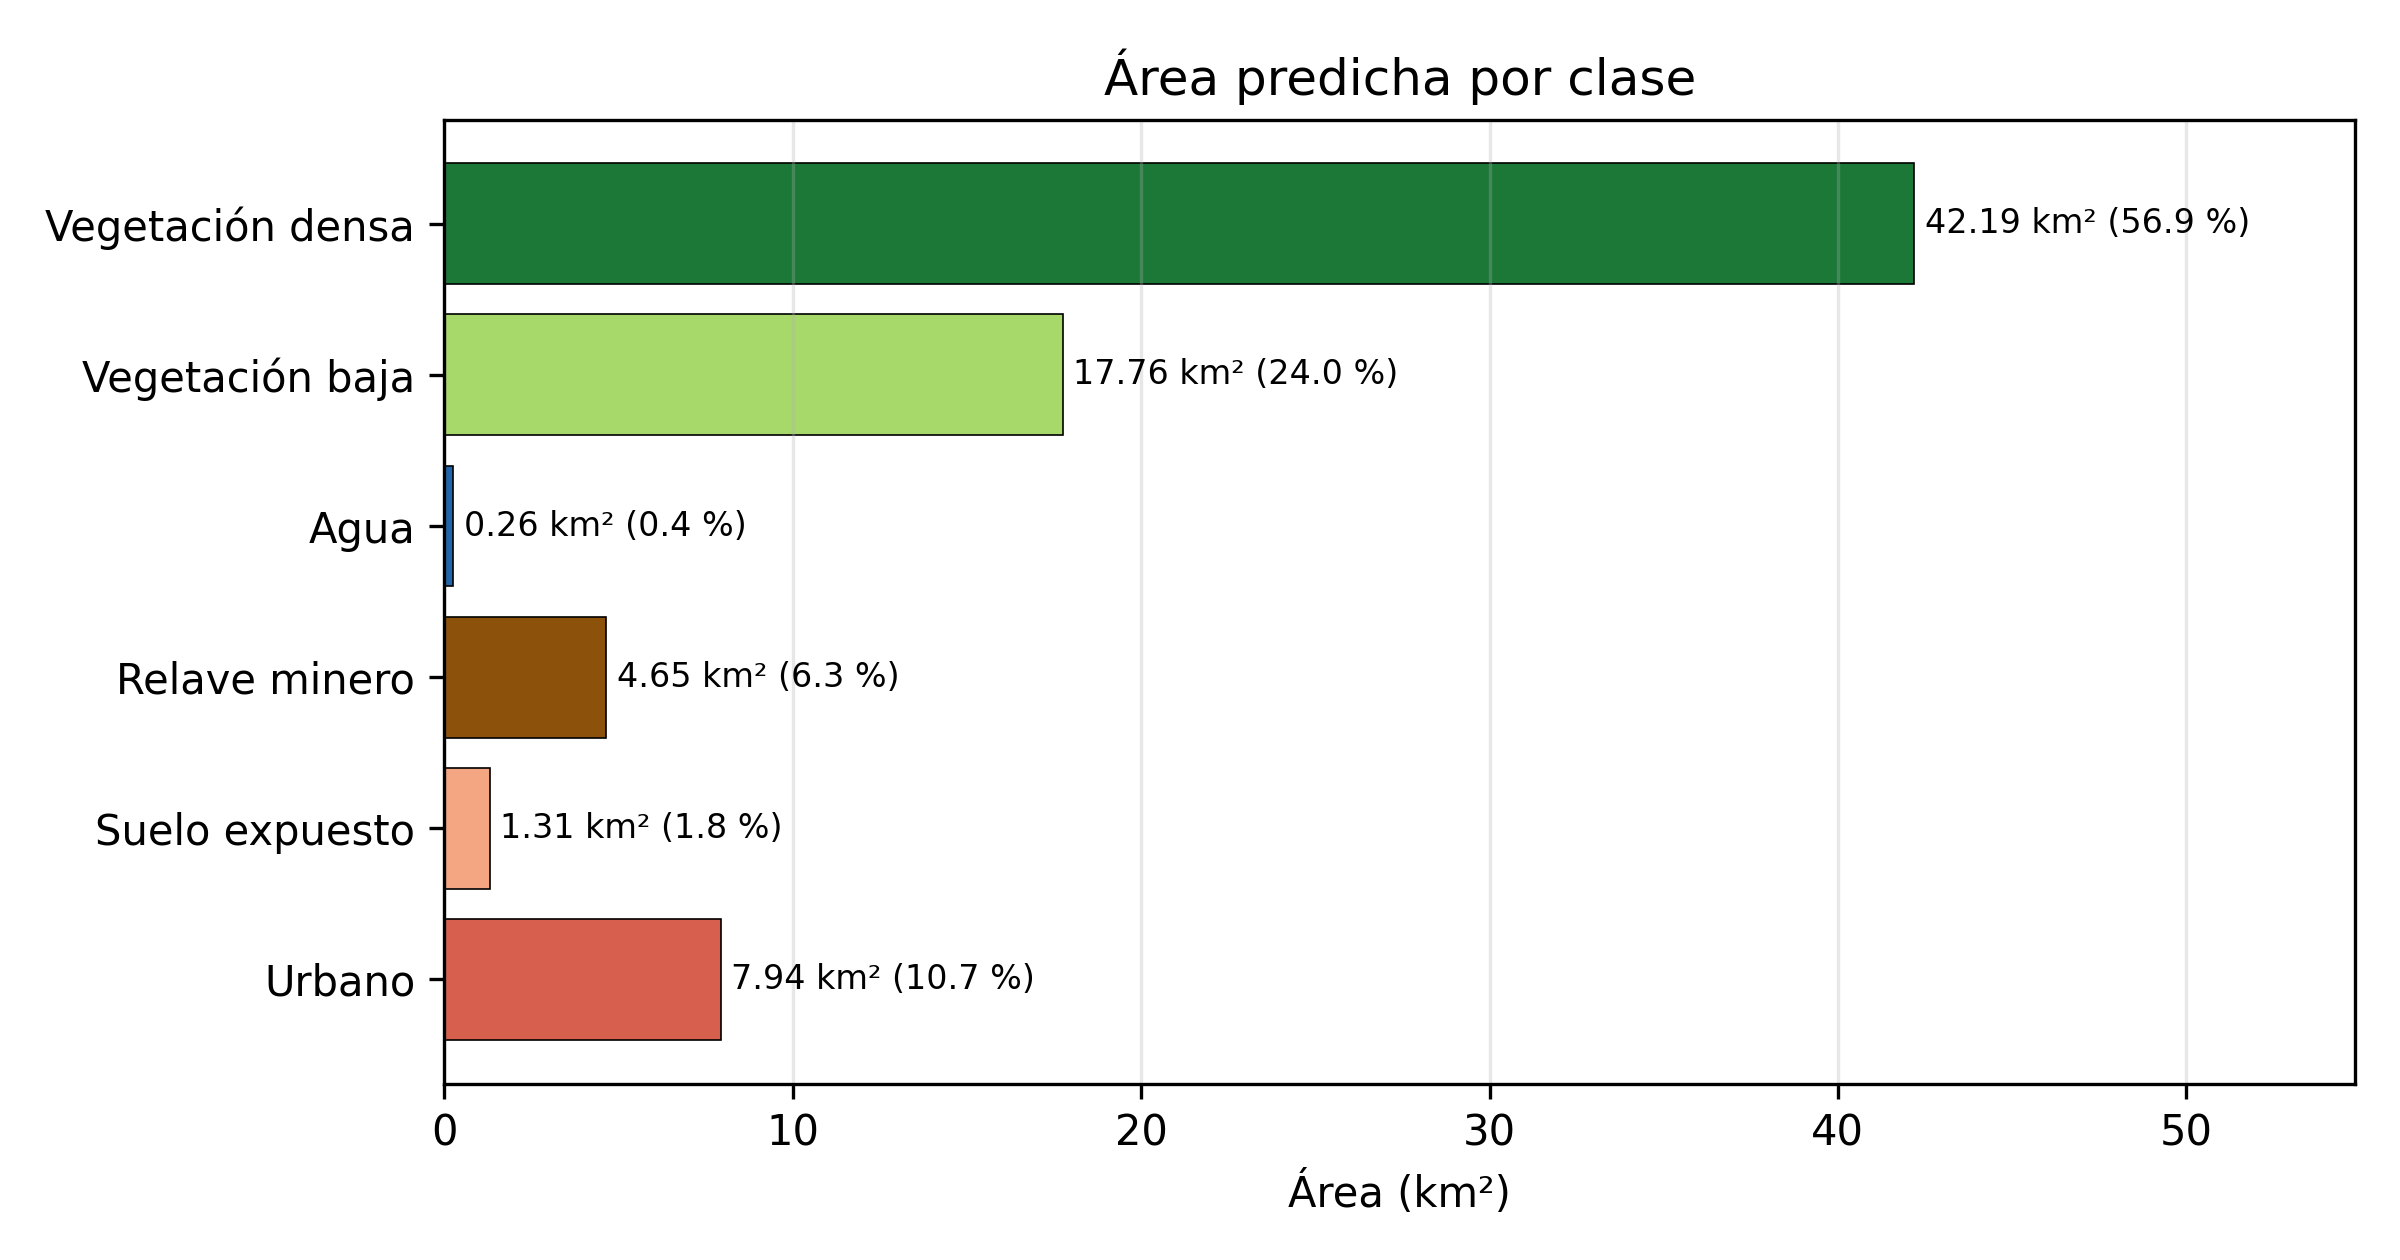
\includegraphics[width=0.85\textwidth]{figures/fase3_area_clases}
 \caption{Área predicha por clase sobre el área válida.}
 \label{fig:f3_area}
\end{figure}

\begin{sloppypar}
La vegetación densa ocupa 42{,}19\,km$^2$ (56{,}9\,\% del área válida), la vegetación baja 17{,}76\,km$^2$ (24{,}0\,\%), el urbano 7{,}94\,km$^2$ (10{,}7\,\%), el relave 4{,}65\,km$^2$ (6{,}3\,\%), el suelo expuesto 1{,}31\,km$^2$ (1{,}8\,\%) y el agua 0{,}26\,km$^2$ (0{,}4\,\%).
\end{sloppypar}

La clase relave requiere una lectura cuidadosa. El corredor del relave tiene 5{,}38\,km$^2$; el modelo predice 2{,}85\,km$^2$ de relave dentro del corredor y 1{,}80\,km$^2$ fuera. El área total de 4{,}65\,km$^2$ no debe interpretarse como el volumen o la extensión oficial del lodo: el modelo confunde parte de las superficies mineras desnudas con relave. La Tabla~\ref{tab:area_corredor} separa la predicción dentro del corredor.

\begin{table}[htbp]
 \centering
 \small
 \setlength{\tabcolsep}{4pt}
 \caption{Área predicha dentro del corredor del relave. El corredor tiene 5{,}38\,km$^2$; el resto de la clase relave queda fuera de sus límites.}
 \label{tab:area_corredor}
 \begin{tabular}{lcc}
  \toprule
  Clase & Píxeles & km² \\
  \midrule
  Vegetación densa & 19.516 & 1{,}952 \\
  Vegetación baja & 2.277 & 0{,}228 \\
  Agua & 828 & 0{,}083 \\
  Relave minero & 28.537 & 2{,}854 \\
  Suelo expuesto & 885 & 0{,}088 \\
  Urbano & 1.675 & 0{,}168 \\
  \bottomrule
 \end{tabular}
\end{table}


\section{Discusión}

El mapa es coherente con la escena: la vegetación domina el área, el urbano se concentra en el casco de Brumadinho, el agua aparece en lagunas y cauces, y el relave sigue el valle del Ribeirão Ferro-Carvão. La separación de vegetación, agua y relave es alta en el test. La dificultad está en suelo expuesto y urbano: sus firmas son parecidas y, a 10\,m, un polígono de suelo puede contener lotes, vías o materiales de construcción. El error de \texttt{5\_06} es consistente con esa ambigüedad: no es un píxel aislado, es un polígono completo.

La ampliación del dataset no mejora de forma demostrable el desempeño. El mejor resultado de la Fase~3 sigue siendo 94{,}7\,\% de exactitud y 0{,}935 de Kappa, igual que la línea base de la Fase~2. La búsqueda de hiperparámetros encontró configuraciones con Kappa de validación más alto, pero no generalizaron mejor al test. En un conjunto de 24 polígonos, una diferencia de uno o dos polígonos cambia varios puntos porcentuales.

Quedan limitaciones importantes:

\begin{itemize}
 \item las etiquetas son pseudo-etiquetas construidas con reglas espectrales y revisión visual, no verdad de campo;
 \item los 72 polígonos originales y los candidatos de suelo no tuvieron revisión individual;
 \item el test tiene solo 24 polígonos y los intervalos bootstrap son amplios;
 \item cinco polígonos añadidos quedaron a 10--60\,m de polígonos de prueba, por debajo de la separación mínima de la Fase~1;
 \item el mapa usa una sola fecha y una sola escena; no captura cambios temporales ni valida la persistencia de las clases;
 \item la clase relave se confunde con superficies mineras desnudas fuera del corredor.
\end{itemize}

\section{Conclusiones}

\begin{enumerate}
 \item La regresión logística regularizada con pesos balanceados fue el modelo más estable; su test es 0{,}947 de exactitud y 0{,}935 de Kappa.
 \item El HPO no produjo una mejora demostrable frente a la Fase~2; el valor de la fase está en el protocolo de selección y en la inferencia completa, no en un aumento artificial de las métricas.
 \item El GeoTIFF temático conserva la grilla, el CRS y el \emph{transform} de la imagen, y puede abrirse y simbolizarse en QGIS.
 \item El área válida es 74{,}10\,km$^2$; la vegetación densa y baja dominan, y el relave predicho es 4{,}65\,km$^2$, de los cuales 2{,}85\,km$^2$ están dentro del corredor.
 \item La estimación de relave y suelo es la parte más débil del mapa; antes de usarla como inventario se necesita verdad de campo y una revisión de las etiquetas.
\end{enumerate}

\section{Reproducibilidad}
La imagen de doce bandas, la capa SCL y los polígonos de entrenamiento se conservan como insumos del proyecto. A partir de ellos, el conjunto de datos, los modelos, las figuras, las tablas y el GeoTIFF se generan con scripts de Python sobre un único entorno reproducible descrito en \texttt{requirements.txt}. QGIS se usa solo para la simbolización y exportación del mapa final (Tabla~\ref{tab:scripts}).

\begin{table}[htbp]
 \centering
 \caption{Scripts del proyecto.}
 \label{tab:scripts}
 \begin{tabularx}{\textwidth}{llX}
  \toprule
  Script & Fase & Función \\
  \midrule
  \texttt{01\_extract\_tsv.py} & 1 & Extrae los píxeles dentro de los polígonos y escribe el archivo TSV. \\
  \texttt{01b\_polygon\_dataset.py} & 1 & Agrega cada polígono (mediana, IQR e índices) y hace el control de calidad. \\
  \texttt{02\_figures.py} & 1 & Genera las figuras y tablas de la Fase~1. \\
  \texttt{03\_train\_models.py} & 2 & Divide por polígono, entrena las pistas A y B y calcula las métricas. \\
  \texttt{04\_phase2\_figures.py} & 2 & Genera las figuras y tablas de la Fase~2. \\
  \texttt{04b\_expansion\_comparison.py} & 2 & Regenera la comparación entre 72 y 88 polígonos. \\
  \texttt{05\_tune\_models.py} & 3 & HPO agrupado, selección, test y modelo final. \\
  \texttt{06\_predict\_raster.py} & 3 & Inferencia por bloques, GeoTIFF y áreas. \\
  \texttt{07\_phase3\_figures.py} & 3 & Figuras y tablas de la Fase~3. \\
  \texttt{07b\_qgis\_map.py} & 3 & Proyecto QGIS y mapa temático. \\
  \texttt{08\_validate\_phase3.py} & 3 & Validación del split, modelo, ráster y áreas. \\
  \bottomrule
 \end{tabularx}
\end{table}

Los comandos son:

\begin{verbatim}
run.bat src\05_tune_models.py
run.bat src\06_predict_raster.py
run.bat src\07_phase3_figures.py
run_qgis.bat src\07b_qgis_map.py
run.bat src\08_validate_phase3.py
latexmk -pdf -interaction=nonstopmode -halt-on-error main.tex
\end{verbatim}

Los artefactos principales son:
\begin{itemize}
 \item \texttt{models/final\_model.joblib} y \texttt{models/model\_card.json};
 \item \texttt{data/prediction/landcover\_lr.tif};
 \item \texttt{data/prediction/landcover\_lr.qml};
 \item \texttt{results/phase3\_*.csv}.
\end{itemize}
La imagen original, la SCL y los polígonos se conservan en \texttt{data/}.

\printbibliography

\end{document}
